\documentclass[12pt,twoside,notitlepage]{report}

%\usepackage{natbib}
\usepackage{a4}
\usepackage{verbatim}
\usepackage{xspace}
\usepackage{graphicx}
\usepackage{float}
%\usepackage{epstopdf}
\usepackage[justification=centering]{caption}
\usepackage{hyperref}

\input{epsf}


\raggedbottom
\sloppy
\clubpenalty1000%
\widowpenalty1000%

\addtolength{\oddsidemargin}{6mm}
\addtolength{\evensidemargin}{-8mm}

\renewcommand{\baselinestretch}{1.1}

\setlength{\parindent}{0.0in}
\setlength{\parskip}{12pt}


% This is a hack to make the appendix in the proposal work.
\makeatletter
\renewenvironment{thebibliography}[1]{%
%     \section*{\refname}%
%      \@mkboth{\MakeUppercase\refname}{\MakeUppercase\refname}%
      \list{\@biblabel{\@arabic\c@enumiv}}%
           {\settowidth\labelwidth{\@biblabel{#1}}%
            \leftmargin\labelwidth
            \advance\leftmargin\labelsep
            \@openbib@code
            \usecounter{enumiv}%
            \let\p@enumiv\@empty
            \renewcommand\theenumiv{\@arabic\c@enumiv}}%
      \sloppy
      \clubpenalty4000
      \@clubpenalty \clubpenalty
      \widowpenalty4000%
      \sfcode`\.\@m}
     {\def\@noitemerr
       {\@latex@warning{Empty `thebibliography' environment}}%
      \endlist}
\makeatother


\newcommand{\texas}{Texas Hold~`em\xspace}
\newcommand{\texasp}{\texas Poker\xspace}
\newcommand{\pa}{Poker Academy\xspace}
\newcommand{\pap}{\pa Pro\xspace}
\newcommand{\mcts}{Monte Carlo Tree Search\xspace}
\newcommand{\sbt}{SimpleBot\xspace}
\newcommand{\sbts}{SimpleBot's\xspace}
\newcommand{\mbt}{MCTSBot\xspace}
\newcommand{\mbts}{MCTSBot's\xspace}
\newcommand{\meer}{Meerkat~API\xspace}
\newcommand{\gs}{GameState\xspace}
\newcommand{\gr}{GameRecord\xspace}
\newcommand{\grs}{GameRecords\xspace}
\newcommand{\pr}{PlayerRecord\xspace}
\newcommand{\prs}{PlayerRecords\xspace}
\newcommand{\player}{Player\xspace}
\newcommand{\opp}{OpponentNode\xspace}
\newcommand{\opps}{OpponentNodes\xspace}
\newcommand{\choice}{ChoiceNode\xspace}
\newcommand{\choices}{ChoiceNodes\xspace}
\newcommand{\chance}{ChanceNode\xspace}
\newcommand{\chances}{ChanceNodes\xspace}
\newcommand{\playern}{PlayerNode\xspace}
\newcommand{\playerns}{PlayerNodes\xspace}
\newcommand{\leaf}{LeafNode\xspace}
\newcommand{\leafs}{LeafNodes\xspace}
\newcommand{\rootn}{RootNode\xspace}
\newcommand{\wf}{WekaFormat\xspace}
\newcommand{\wfs}{WekaFormats\xspace}

\begin{document}


%%%%%%%%%%%%%%%%%%%%%%%%%%%%%%%%%%%%%%%%%%%%%%%%%%%%%%%%%%%%%%
% Title


\pagestyle{empty}

\hfill{\LARGE \bf David Moody}

\vspace*{55mm}
\begin{center}
\Huge
{\bf Monte Carlo Tree Search in \\\texasp} \\
\vspace*{5mm}
Computer Science Tripos, Part II \\
\vspace*{5mm}
Christ's College \\
\vspace*{5mm}
\today  % today's date
\end{center}

\cleardoublepage


%%%%%%%%%%%%%%%%%%%%%%%%%%%%%%%%%%%%%%%%%%%%%%%%%%%%%%%%%%%%%%
% Proforma, table of contents and list of figures

\setcounter{page}{1}
\pagenumbering{roman}
\pagestyle{plain}

\chapter*{Proforma}

%{\large
\begin{tabular}{ll}

Name:				& \bf David Moody \\
College:			& \bf Christ's College \\
Project Title:		& \bf Monte Carlo Tree Search in \texasp \\
Examination:		& \bf Computer Science Tripos, Part II, 2010-2011 \\
Word Count:			& \bf Approximately 12,000 words \\
Project Originator:	& Dr Sean Holden/David Moody \\
Supervisor:			& Dr Sean Holden \\ 

\end{tabular}
%}

\stepcounter{footnote}


\section*{Original Aims of the Project}

To build a computer poker player using the \mcts algorithm. The program should also implement an opponent model and have a variety of different strategies to choose from. It should be able to consistently beat an existing simple opponent, \sbt.


\section*{Work Completed}

I have successfully implemented the program as originally intended. It can play as well as I had expected and can consistently beat \sbt.
% I have completed all of my original success criteria. 
All work completed is described in this dissertation. 


\section*{Special Difficulties}

None.

 
\newpage
\section*{Declaration}

I, David Moody of Christ's College, being a candidate for Part II of the Computer Science Tripos, 
%[or the Diploma in Computer Science], 
hereby declare that this dissertation and the work described in it are my own work, unaided except as may be specified below, and that the dissertation does not contain material that has already been used to any substantial extent for a comparable purpose.

\bigskip
\leftline{Signed }

\medskip
\leftline{Date }

\cleardoublepage

\tableofcontents

\listoffigures

%\newpage
%\section*{Acknowledgements}
%TODO: There are none?


%%%%%%%%%%%%%%%%%%%%%%%%%%%%%%%%%%%%%%%%%%%%%%%%%%%%%%%%%%%%%%
% The Chapters

\cleardoublepage
\setcounter{page}{1}
\pagenumbering{arabic}
\pagestyle{headings}


\chapter{Introduction}
\section{My Project} 							% ----

% Is this a good section title?
% What was I trying to do?
% Mention \pap and \sbt.

My project was to build a program to play \texasp. The program uses the \mcts algorithm for searching large trees. It also incorporates an opponent model to assist in the presence of hidden information. I have successfully implemented the program as originally intended. It can play to an acceptable level and can consistently beat a simple opponent I chose in my original plan, \sbt. The program and this dissertation successfully complete all of my original success criteria. However, I did not have time to complete any of my planned extensions.


\section{The Game of Poker}						% ----

% Very brief intro to the rules of poker, mention the appendix A where a more detailed explanation is given.
% Why poker is challenging for computers.
% Poker is a card game. 2+ players. Objective is to win money, can be done by winning hands, that is done by being the only player left in the game or by having the best hand at the end of the game. Three possible actions, raise, call or fold. 
% Why did I choose limit \texasp.

% Mention other poker bots briefly. Say the phrase poker bot.
% Briefly talk about the methods used by them.
% Mention \sbt.
% Talk about the one that I have been roughly following.

Poker is a game of imperfect information, where the other players know different things and may try to deliberately mislead you. There is also an element of chance in what cards will come up next. In addition, there can be as many as 10 players in a game which can result in an enormous number of possible game states. These things make it particularly difficult for computers to play poker. 

Despite this, there have been many successful attempts to build competent computer poker players (aka poker bots). Here is a brief overview of just a handful of them:
\begin{itemize}
\item Poki, 1999: A full-ring limit poker bot, its main problem was that it could not adapt its strategy fast enough to prevent its own exploitation~\cite{poki}.
\item PsOpti, 2002: A heads up limit poker bot, built using a game theoretic approach~\cite{psopti}.
\item Vexbot, 2003: A heads up limit poker bot which uses opponent modelling and the expectimax algorithm to adapt to its opponents~\cite{vexbot}.
\item Polaris, 2007: Another heads up limit poker bot which contains a number of different strategies and chooses between them during a match~\cite{polaris}.
\end{itemize}

%The last one 



\section{\mcts}									% ----

% When/why is mcts used.
% Why is it needed here.
% Brief description of stages.
% Brief description of strategies.

\mcts is a best first search technique used to search very large trees.
% which may be too large search exhaustively. 
It uses stochastic simulations to help decide which action to take. It tries to focus its simulations onto the branches which it thinks will be most relevant, assuming all players play rationally. Every time it simulates a game, it backpropagates the result back through the tree so that it can make better decisions about which game to simulate next.

MCTS has been successfully been applied to Go \cite{mcts-go}, Backgammon \cite{mcts-bg}, Limit and No-Limit \texas \cite{mcts-iomp} \cite{mcts-erd} as well as several other games. 
% Something about how great mcts is. 

In this project I will be using MCTS with a variety of different strategies. In the evaluation, I will compare the effectiveness of some of the different strategies and see how varying the thinking time affects performance.




\section{Opponent Modelling}					% ----

% Discovered that it is needed, at least the way in which I'd done it.
% What is Weka?
% Where did I get training data from.

An opponent model can be used to predict the cards that the opponents hold and the actions they will take. There has been quite a lot of research on different opponent modelling techniques in poker including some models which can dynamically adapt to different players. 
% Cite that?

In this project, I will be using relatively simple opponent models which use classifiers created by an open source machine learning library called Weka. My approach is similar to that taken by \cite{mcts-erd}.
% TODO: make the reference look better.

I eventually found that opponent modelling is very important to the success of the program. Without it, the program was not able to beat \sbt.



\section{Results}								% ----

% Project went well.
% Completed all of the success criteria in the original proposal.

%Overall, I would say that my project was definitely a success. 
The project has been a great success.
The program is able to beat the simple opponent originally proposed in the project proposal, \sbt. It can also be the most successful player when played against three separate instances of \sbt. I have also shown how varying different factors, such as the thinking time or the presence of the opponent models, affects performance.

The program and this dissertation complete all 7 of my original success criteria. 




%\section{Summary}								% ****

% Recap of why poker is difficult.
% Recap of why mcts is used.
% Recap of why opponent modelling is needed.
% Recap of success.
% What did I set out to do?

%TODO: recap of this chapter



\cleardoublepage
\chapter{Preparation}
\section{The Rules of Poker}					% ----

% 2+ players.
% Each player has 2 cards only they can see.
% Round of betting, 3 community cards, round of betting, 1 community card, round of betting, 1 community card, round of betting. Winner takes pot/winners split pot.
% Description of a betting round.
% Some basic strategy.
% Mention the appendix A for more on the rules of poker.
% Mention the different variations of poker and why I chose \texas.


To help you better understand this project, I will now briefly explain the rules of Limit \texasp. 
%A more detailed explanation can be found at the end, in \hyperlink{rulesoftexas}{Appendix A}. 

There is a minimum of two players and usually no more than ten. At the start of each game, each player is dealt two cards, face down so that only they can see them. These cards are often called the hole cards.

Then there is a round of betting. In a round of betting, going clockwise through the group starting with the player to the left of the dealer, each player must choose to perform one of the following possible actions: they can fold, and drop out of the game; they can call, and place into the pot the current maximum bet; or they can raise, and increase the current maximum bet by a fixed amount. Note that calling when the current maximum bet is zero is usually called checking. The betting round continues until all players have either folded or matched the current maximum bet. 

Here is a quick example betting round between three players, Alice, Bob and Charlie:\\
\begin{center}
\begin{tabular}{c|c|c|c|c}
Player & Action & Amount in pot from & Total amount in pot & Current \\
 & & player before/after & before/after & maximum bet \\
\hline
Alice   & Check & \$0 / \$0 & \$0 / \$0 & \$0 \\
Bob     & Raise & \$0 / \$1 & \$0 / \$1 & \$1 \\
Charlie & Call  & \$0 / \$1 & \$1 / \$2 & \$1 \\
Alice   & Raise & \$0 / \$2 & \$2 / \$4 & \$2 \\
Bob     & Call  & \$1 / \$2 & \$4 / \$5 & \$2 \\
Charlie & Fold  & \$1 / \$1 & \$5 / \$5 & \$2 \\
\end{tabular}
\end{center}

After this round of betting, if at least two players are still in the game, three cards are dealt face up onto the table. There is another round of betting, another card on the table, another round of betting, a final card on the table and then a final round of betting. The four betting rounds are usually given the following names: preflop, flop, turn and river.

If all but one of the players folds then the remaining player takes all of the money in the pot. If the final betting round has ended and there are still two or more active players then there is a showdown; all active players show their cards and the player who can make the best poker hand wins the pot. It is also possible for multiple players to be able to make the same best poker hand. In this case, they will each take an equal share of the pot.

The best poker hand of each player is made up of the best combination of their two hole cards and the five cards on the table. The exact ranking of a poker hand is quite complicated and not really necessary to know for this project so I will not describe it in any more detail. All you need to know is that there are relatively fast algorithms for finding a numerical rank of a poker hand such that any better hand will have a higher rank, any worse hand will have a lower rank and any equal hand will have the same rank.

In Limit \texas, the small bet is the amount that one is allowed to increase the current maximum bet by (in the first two betting rounds). In the above example the small bet is \$1. In the last two betting rounds, the amount that one is allowed to increase the current maximum bet by is usually doubled (to \$2 in this example). To avoid any confusion, throughout this project the small bet will always be equal to \$1. Also there is a limit to how large the current maximum bet can be. The limit is usually four times the raise increment (so \$4 in the first two rounds of betting and \$8 in the last two). This puts a limit on length of the game. 

In the first round of betting (preflop) there is an additional rule. The player to the left of the dealer must place into the pot the small blind and the player to the left of that player must place into the pot the big blind. These blinds are similar to regular bets except they are not optional. The small blind and big blind are usually equal to one half of the small bet and one small bet respectively. The main purpose of the blinds is to get the betting going and prevent the players from all checking in the first round. Also, if no one else raises in the round then the player who put in the big blind is given the opportunity to raise.

There are a lot of complex rules regarding what to do when a player has run out of money but is still in the game. However these situations are very rare so I will not consider them.

There are many other varieties of poker including one where players can raise any amount they want. The reason I chose Limit \texas is because \texas is the most popular variety (and is the version I play) and because designing a No-Limit bot would have been too complicated. Also note that throughout the project, I will be referring to cash games as opposed to tournament games.

%Also note that throughout the project, I will always be talking about cash games as opposed to tournament games. The difference is that in cash games, winning \$10 will always be worth the same no matter how much money you already have. However in tournament games, winning \$10 when you only have \$5 left is worth more to you than if you had \$500 left. I chose to use cash games because it makes the strategy simpler and it means that I didn't have to simulate complete tournaments to get results. 



\section{\pap}									% ----

% What is it? It's not free. Graphical user interface. Provides the framework for playing poker bots against themselves. The statistics tracking abilities it has.
% Why other people use it and why I'm using it.
% The meerkat API.
% The flaws of \pa.
% The alternative to using \pap. Open Test Bed. Why I chose not to use it and if I regret my decision. What I would have done if I had used it. How the project would have been different if I had used it.
% Screenshots(?)


\pap \cite{pa} is a commercial program\footnote{It costs \$85 from the \pa website.} which provides a variety of useful and fun features for playing and analysing poker games. The two features that are relevant for this project are: the ability to play user created custom poker bots against a variety of existing poker bots; and the ability to record and analyse various statistics about the games played.

The \meer \cite{meer} provides the ability to create a plug-in bot which can play in the \pa program; all that is required is to create a Java class that implements a given interface.
% and you should be ready to go. 

I chose to use \pa because of the graphical user interface, because of its statistics tracking capabilities and because it was highly recommended. There were two alternatives. The first was to write the code for simulating the games myself. This would have been very difficult and would have taken too long.
The second possibility would have been to use opentestbed \cite{opentestbed}. Opentestbed is an open source implementation of the \meer for running poker games. In retrospect, I think it would have been better to use opentestbed. It was designed specifically for the purpose of testing poker bots and may have been easier to use. 
%However, I didn't use it.\footnote{Also it would be quite tricky to port my current program to it because my current program uses two important classes in the \meer which are not included in opentestbed.}

\begin{figure}[h!]
\centering
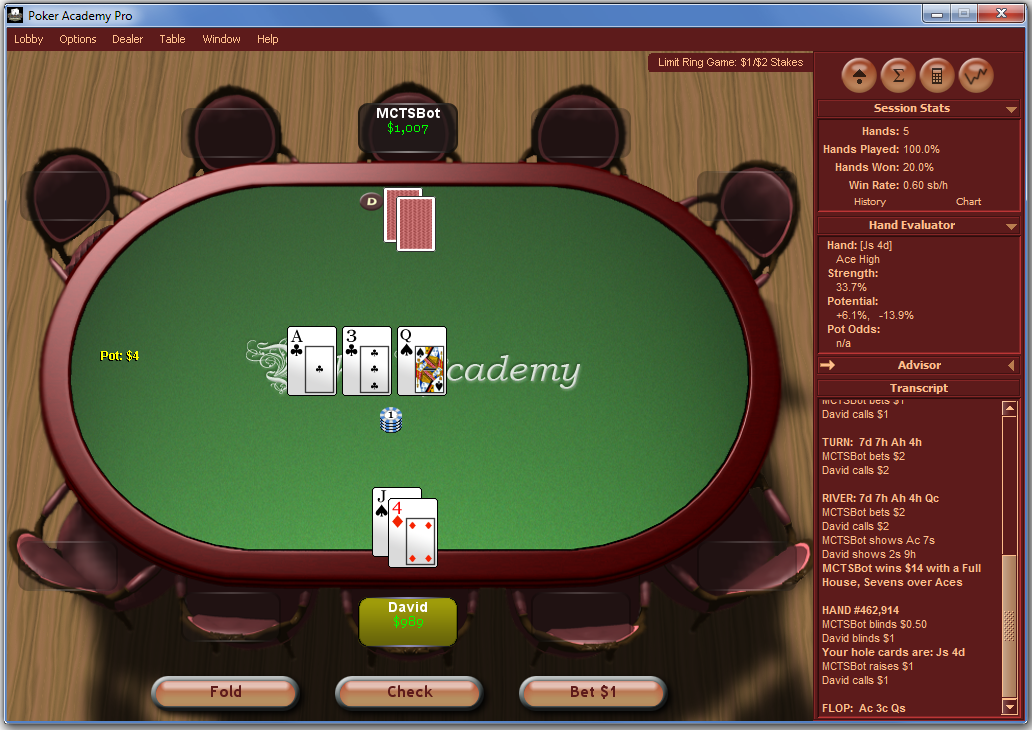
\includegraphics[width=144mm]{Screenshots/PAP1.png}
\caption{A screenshot of \pap.}
\end{figure}

%\begin{figure}[h!]
%\centering
%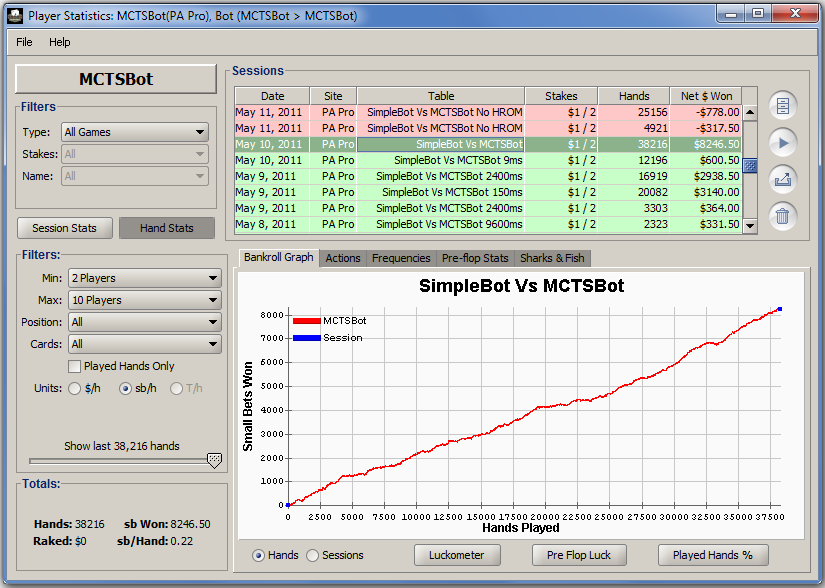
\includegraphics[width=144mm]{Screenshots/PAP2.png}
%\caption{Another screenshot of \pap.}
%\end{figure}



\section{\sbt}									% ----

% \sbt, what is it, how well does it play, and why am I using it?
% Where did it come from?
% The alternatives to using \sbt. I didn't want to compete.
% Attach the complete source code of \sbt?

 
%The source code for \sbt can be found in 
%Appendix \ref{app:sbsource}.
%\hyperlink{simplebotsourcecode}{Appendix B}.


\sbt is an example poker bot provided with the \meer. The important points to note about \sbt are:
\begin{itemize}
\item It only considers its own hole cards, the table cards, the amount in the pot and the number of active players.
\item It ignores the past actions of all players.
\item It is non-deterministic and has the ability to bluff.
\end{itemize}

\sbts playing ability is not comparable to that of an experienced human's, however it is good enough to provide a challenge for another poker bot. 

I chose to use \sbt as the opponent to test and evaluate my program against throughout the project. I did this because I needed an opponent to test against and I didn't want to be in competition with some of the really strong poker bots that have been in development for years. Thus, I settled on \sbt, a good enough opponent to provide a challenge but not so good that 
%I wouldn't be able to succeed.
I wouldn't stand a chance.

%The \sbt source code also helped me to understand some of the features of the \meer and was very useful when creating my program. 



\section{The Game Tree}							% ----

% This used to be in the imp.

% What is a game tree in general and why is it needed for the \mcts algorithm?
% What is it in this case, i.e. what are the nodes in the tree and what order/structure is there.
% Make a diagram of a game tree?
% Make distinction between the stored game tree and the full game tree.
% Choice nodes: Your turn, need to choose an action, root node is always a choice node.
% Opponent nodes: an opponent's turn, need to model them to see what they will do next.
% Chance nodes: Betting round has just finished and new cards are about to be drawn. Mention that there can be many possible children when three cards are to be drawn and how I got around it.
% Leaf nodes: The game has just ended. There are several possible cases.
% All opponents folded and you didn't, you win.
% You folded, you lose.
% You didn't fold and at least one other opponent is still in the game, need to guess result from table and betting history.
% Also mention at some point, not necessarily here, that I am modelling cash games not tournament play, and also that there is a limit of 4x the small bet per betting round.

% Make the distinction that I'm now talking about the actual implementation of the nodes rather than the general idea of nodes.
% Introduce the Node abstract class. 
% Stores several things needed by the \mcts algorithm including: visit count, expected value, std dev, etc.
% Mention all of the separate classes for the different nodes and say that more detail is coming in the next section.


%In this section I will explain what a game tree is and how it relates to poker and the MCTS algorithm. I will then go on to describe the different types of node found in the tree.

A game tree is a directed graph where each node represents a possible state in the game. An edge between nodes represents an action that transforms the parent node into the child node. The root node is the initial position and the leaf nodes represent positions in which the game has ended.
%are the final positions in which you either win, lose or draw \cite{gametree}.

For games which have perfect information and no random elements, it is possible to search the tree using the minimax algorithm. 
There are extensions to the minimax algorithm which allow it to deal with random elements (expectiminimax) and larger trees (alpha-beta pruning or limiting depth search combined with an evaluation function).
However, there are a few problems with these methods and they are not always suitable for poker. 

%However, this isn't practical in poker (and so you have to use something else, like MCTS).

%TODO: cite something for this?

%TODO: talk about minimax?

% Add some connecting scentence here?


In the poker game tree, there are several different types of node:
\begin{itemize}
\item Choice node, this is where the next action will be performed by the bot. It can choose to raise, call or fold and the children of this node will reflect the choice that was made.
\item Opponent node, this is where the next action will be made by one of the opponents. They can raise, call or fold. 
\item Chance node, this is where the current betting round has ended and one or more new cards are about to be dealt onto the table. This node can have either 46 or 47 children in the flop or turn stages, where one card is about to be dealt, or 50*49*48=117600 children in the preflop stage, where three cards are about to be dealt. 
\item Leaf node, this is where the game has ended. This node type has no children. There are three possible subtypes of this node:
	\begin{itemize}
	\item All opponents folded, this is where the bot is the only remaining player in the game; it wins by default. 
	\item Bot folded, this is where the bot has folded but other players are still in the game. The game might not necessarily have ended, however since the bot is no longer playing, there is no point in continuing.
	\item Showdown, this is where the bot and one or more other opponents are still playing and the final betting round has ended. In this case, it is not possible to say who wins because there is no way to tell what cards the opponents have. The result of the game has to be estimated from the strength of the best poker hand that the bot can make and the behaviour of the opponents up to this point.
	\end{itemize}
\end{itemize}

%For an example poker game tree between two players, see the following diagram.

%TODO: make diagram.





\section{\mcts}									% ----

% Briefly, what is a game tree?
% Very briefly, what is \mcts.
% Why is it appropriate here?
% The stages:
% Selection: Choose which node to explore. Need to have a good balance between exploration and exploitation. Several possible strategies to use here. Using opponent modelling here.
% Expansion: Generate the new nodes from the current node, generally trivial.
% Simulation: Very complicated part. Many possible strategies to use here. It is important that it is quick and easy to do. Simulate to completion, game cannot go on forever. Always call/others, using opponent modelling here.
% Backpropagation: Update the game tree. Two possible strategies both very similar.
% Repeat until finished.
% Again mention the project that I'm basing mine on.

\label{sec:mcts-prep}

%I will now describe the general \mcts algorithm. In the implementation chapter, I will go into more detail about how it relates to poker and about the specific strategies that I used.

The \mcts algorithm gradually builds up a subsection of the full game tree by starting at the root node and adding a new node in each iteration. The new nodes are not added at random though, the algorithm tries to add more nodes to the tree in places which it thinks are more likely to be relevant.

For example, if an opponent has been raising all game then that opponent is unlikely to fold in the final betting round. Thus the MCTS algorithm will spend more time building the subtrees where the opponent does not fold than the subtrees where the opponent does. 

%Here is another example, if your opponent has been checking all game then they are quite likely to fold if you were to raise. Therefore the algorithm will spend more time on the subtrees where you raise than the subtrees where you call. Of course, the algorithm cannot simply ignore the subtree where you call because it might be possible that, by calling, you could trick your opponent into raising and then re-raise yourself, potentially getting more money than if you had just raised straight away.\footnote{There is however one occasion where you can safely ignore a subtree. When any player has the opportunity to check then you can assume that they will not fold, even though it is a perfectly legal move.}
% Should I include this?

One of the advantages of the MCTS algorithm is that it does not need to search the tree exhaustively and can be halted at any point. This is extremely useful because the full game tree can easily become very large and searching the entire tree could take more time than is available. 




%MCTS is a best-first search method. It works by simulating a large number of games and using the results of those simulations to decide which action to take. The simulations are not done at random though. The algorithm attempts to focus its effort on the simulations which it thinks will be most relevant. It does this by gradually building up a subsection of the full game tree, starting at the root node and adding a new node in each iteration. The new nodes are not added at random though, the algorithm tries to add more nodes to the tree in places that it thinks are more likely to be relevant.

%Instead of searching the whole tree exhaustively, it samples from it. This allows it to work on the very large game trees that can appear in poker. It also allows it to give an estimate in a very short amount of time.


The actual body of the algorithm is fairly simple. It consists of four main stages which are repeated until the program runs out of thinking time. The four stages are:
\begin{enumerate}
\item Selection: Here, starting at the root of the tree, the algorithm selects the next node that it wishes to look at and repeats until it has reached a leaf node of the stored tree. The selection stage focuses the algorithm onto the paths which appear to be the most relevant.
\item Expansion: One (or more) children are then added to the node selected in the last stage.
\item Simulation: The game is simulated (to completion) from the state at the newly added node to attain an estimate for the expected value of the node. 
\item Backpropagation: Once a simulation result has been calculated, the algorithm goes back through the path that had been taken and updates the visit counters and expected values of all of the nodes that it encounters. 
\end{enumerate}

%These four stages are repeated until you run out of thinking time. 
%You then need to select the action that you are actually going to take. This usually involves selecting the one which has the highest expected value. 
%You can select the action which has the highest expected value, you can also select the action which has the highest visit count. In practice, both of these methods usually return similar results. 

Then, the actual action that is to be taken needs to be selected. It is usually the one which has the highest expected value. 


For the selection, simulation and backpropagation stages, there are several different strategies that can be employed. In the implementation chapter, I will describe the strategies which I used and in the evaluation chapter I will compare their effectiveness. 
% Sounds not quite right.



\section{Opponent Modelling}					% ----

% Why is it needed?
% Can you get away with not using it at all?
% Current research on it(?)
% What do I need to predict?
% The probability that an opponent will take a given action. Used in the selection stage to select the next node when looking at an opponent node.
% The result of a simulated game. Used in the simulation stage.
% Why do I need to predict those things? Are there alternatives?
% How am I actually going to predict those things? Use Weka.

Opponent modelling is where one attempts to create a model to predict certain information about ones opponents. Two useful things that can be predicted are:
\begin{enumerate}
\item The hand rank of the best poker hand an opponent can make given the cards on the table and the opponent's previous actions.
\item The probability that an opponent will perform a given action at a particular stage given the cards on the table and the opponent's previous actions.
\end{enumerate}

The first can be useful when trying to predict the result of a simulated game and the second can be useful when selecting the next node to examine (where the next action will be made by an opponent). Without an opponent model, a variety of different problems can occur. For example, if an opponent is showing signs of weakness then it is often a good move to raise and force them to fold. However, if an opponent model is not being used then this option may be overlooked.


%For example, it could be difficult to tell when your opponent had a strong hand so you might keep raising only to be beaten at the showdown.


%Without any kind of opponent model you run into one major problem. The problem is that you have no realistic way of knowing how strong the opponents hand actually is. This can lead to all kinds of problems where you keep raising, only to be beaten at the showdown or fold even though your opponent is showing signs of weakness. 

I found that implementing the opponent model had a major effect on the performance of the program; it was the first thing I did that enabled the program to start beating \sbt.



\section{Weka}									% ----

% What is Weka?
% Why is it good?
% Why am I using it?
% What are the alternatives?
% Mention having to use an older version for compatibility.
% ARFF, what is it, why do I need it, alternatives?


Weka (Waikato Environment for Knowledge Analysis) \cite{weka} is a collection of machine learning algorithms written in the Java programming language. Weka is available under the GNU General Public License.

Weka provides several features that I needed for this project. The most important is the ability to create classifiers for use in the opponent models. It also provides a useful GUI to help in analysing the training data and creating the classifiers.
%(see figure \ref{screenshot:weka} for a screenshot). 
Weka has been used for creating opponent models in similar poker bots \cite{mcts-erd} so I was confident that it would work here.

\begin{figure}[h!]
\centering
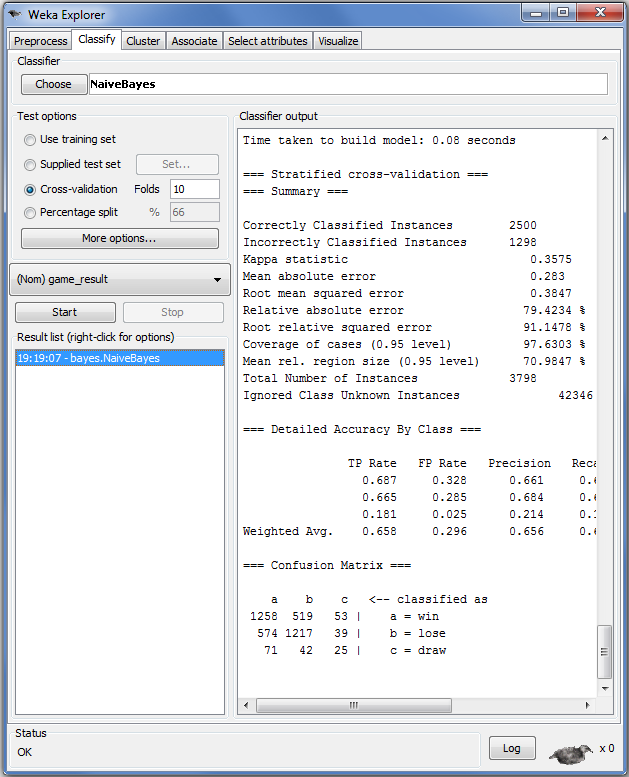
\includegraphics[width = 5.6in]{Screenshots/Weka.png}
\caption{A screenshot of the Weka Explorer.
%\\ useful for visualising ARFF files and trying out classifiers.
}
\label{screenshot:weka}
\end{figure}

The alternatives to using Weka would have been to create my own machine learning algorithms, which I did not have time to do, or to use a different software package, for example Matlab. In the end I chose to use Weka because it runs on Java, which is also used by \pap, and because it looked easy to use. 

Note that even though Weka produced the classifiers, I still had to write a significant amount of code to integrate them into the program.

Unfortunately, because \pa runs with Java 1.5, I was not able to use the most recent version of Weka and had to use an older version from 2004 (version 2.3.3). I doubt this had much of a negative effect on the project as version 2.3.3 had all the required features. 




\section{Training Data}							% ----

% Needed by Weka.
% Mention that game records are called hand histories.
% Originally intended to get it from a source on the web (cite them).
% Realised that I could just as easily get it by playing \sbt against itself in \pa.
% Still haven't looked at the online data.
% Also tried using data gathered by playing \sbt against \mbt once I had a working program. Didn't provide much of a difference.
% Mention the problem of converting the hh's into something that Weka can recognise.
% \pa exports and the internet hh's come in plain text human readable descriptions. 
% I planned to do it by writing a tool to convert them into arff.


In order for Weka to create a classifier, it needs to be provided with training data. In this case, training data takes the form of records of played games (called hand histories). I had originally planned to get hand histories from a source on the internet \cite{dataminedhhs}. I eventually realised that I could get hand histories more easily by playing \sbt against another instance of itself inside \pap. Early on in the project, I set up a match of \sbt Vs. \sbt and let it run for 50,000 games. I used that as the training data for all of the classifiers I created.

There is also a problem of converting the hand histories into a format that Weka can recognise. Hand histories exported from \pa (or from the web) come as human readable plain text descriptions of the games. Before I could use them as training data for Weka, I first had to convert them into Attribute Relation File Format (ARFF). I wrote my own tools to do this as there are no freely available ones. 
%I ended up spending a lot of time experimenting with different ways of representing the hand histories.



\section{The Plan}								% ----

% First the basic classes and logic.
% Next the \mcts algorithm.
% Next the opponent model.
% Explanation of why in that order.
% Explain about how you can easily change the strategies used.
% Mention the full original plan in the appendix.
% Evidence of good software practice?
% Something about design specifications?

% What I originally planned to do.
% Improving simulation and selection strategies.
% Improving the predictive capabilities of the opponent models.
% Adapt on the fly to new and different opponents. Not done because I didn't really have any different opponents to play against.

% Requirements analysis, or something else?

In my original plan, I proposed to complete the work in the following order:
\begin{enumerate}
\item Create the basic classes needed, implement the game logic and integrate with \pap.
\item Implement the framework for the MCTS algorithm and create basic strategies.
\item Implement more complex strategies for the MCTS algorithm. 
\item Collect and consolidate hand histories. 
\item Use Weka to create opponent models and integrate them into the main program.
\item Evaluation and testing. 
\end{enumerate}

%Part of the reason I chose to do it in this order was that it meant I would be able to have a working poker bot half way through the project. 

I chose to do it in this order because it allowed me to produce a working poker bot after the first term. It would have also allowed me to complete the project without the opponent model if the implementation of the MCTS algorithm had taken too long. 


Throughout the project, I was using Mercurial for version control and Dropbox to backup the repository. I had also intended to write good documentation for all of the classes in the project\footnote{However, due to time constraints, I was not always able to do this.}.



%If I had completed all of that and still had time to do more, I was going to attempt the following extensions:
%\begin{enumerate}
%\item Making the opponent models adapt to specific players on the fly.
%\item Try out some more elaborate simulation and selection strategies. 
%\item 
%\end{enumerate}

%In the end, I didn't have time to complete any of these. 

% TODO: add more?



























\cleardoublepage
\chapter{Implementation}
\section{Integration With \pap}					% ----

% Recap of what \pap is and why I'm using it.
% Recap/introduction to the \meer.
% Mention some of the problems with the \meer and mention the alternative again.
% Mention the \sbt example and how it helped me.
% Include the full \sbt code in the appendix and mention it?

% Now talk about the details.
% My class, \mbt implements the Player interface.
% Must implement several methods:
% void init(Preferences prefs)
% void holeCards(Card c1, Card c2, int seat)
% Action getAction()
% Also several from GameObserver which are all void and which allow you to observe the things that happen in the game. Some were needed but some weren't.
% Give examples and more detail.

% Talk about the GameInfo object and how it is used to get information about the game state, say why I didn't use it in the main part.
% Mention some of the shortcomings of the API, including the problems I had. e.g. the use of seat numbers, the weird blinds for 2 people, etc.
% Talk about the Card and Hand classes and about the Deck and HandEval classes. Why did I use them and what were the alternatives.
% Should this go in the preparation chapter?


One of the first challenges I faced was getting my program to correctly interface with \pap. In this section I will briefly discuss how I did this and give a quick description of some of the useful features of the \meer.

Recall that \pa allows users to create their own plug-in bots. To do this, the \meer is required. The \meer contains an interface called \player which all plug-in bots must implement. My bot, which is called \mbt, implements the \player interface.

I will not describe the API in great detail but there are three important methods in the \player interface: getAction, this is called every time \pa wants to know what action the bot wants to perform and it is where the majority of the work is done; init, this is called when the bot is first loaded, it allows the bot to initialise itself with some given preferences; and holeCards, which is called once per game to tell the bot what its hole cards are. There are also eight other methods which are used to notify the bot whenever any action occurs in the game. I implemented most of these methods in order to keep a record of the past actions of the other players.


%There are several important methods in the \player interface, the first is getAction() which is called by \pa when it is \mbt{}'s turn and it needs to know what action (raise, call or fold) \mbt wants to take. The majority of the calculation occurs when this method is called. 

%There is an init(Preferences prefs) method which is called when the bot is first loaded. This allows you to customise the parameters of the bot by loading them from a separate file. You could also have multiple bots running from the same source file but with different parameters. In the end, I found it more convenient to simply change the parameters in the source code rather than use this method.

%There is a holeCards(Card c1, Card c2, int seat) method which is called at the start of a hand when you are dealt your cards and assigned a seat number. 

%There are also a bunch of methods in the GameObserver interface (which the Player interface extends) which are called to notify you of certain events that occur during the game. For example: actionEvent(int seat, Action action) which is called whenever any player performs an action; stageEvent(int stage) which is called whenever the game advances to the next stage; gameStartEvent(GameInfo gi) which is called to let you know that a new game has started and to give you the relevant information in the GameInfo object; and 5 others which notify you of other events. I had to implement the 3 that I mentioned in order to keep track of how the game was progressing. 

% Is this too much detail?

%If I had been designing the \meer, I would have done things a bit differently; I would not have included any of the methods from the GameObserver interface and instead I would pass an additional argument to the getAction method. This argument would be an object containing all current relevant information as well as a history of everything that had happened so far in the hand. I think this would be a good idea because it would reduce the complexity of a poker bot, it would reduce the number of empty methods and it would probably reduce the risk of programmer error.
% Is this a good explanation?

%The \meer also provides a few other useful classes: 
%\begin{itemize}
%\item The Card class, this provides a basic representation of a card. I used this class throughout the project.
%\item The Deck class, this provides a way to randomly extract a Card from a set of Cards.
% I could have easily implemented this myself but because it was already here, I decided to use it.
%\item The Hand class, this is a collection of Cards.\footnote{For some unexplained reason, the Hand class indexes its cards starting at 1, I had a lot of problems until I realised this.}
%\item The HandEvaluator class, this class is used for determining the numerical rank of a 5-7 Card Hand. It is one of the most useful features of the \meer.
%\item The Action class, represents an action that a player can take. I ended up making my own action classes although I could have easily used this. 
%\end{itemize}

The \meer also provides a few other useful classes: the Card class, which provides a basic representation of a card; the Deck class which provides an easy way to extract a random Card; the Hand class which is a collection of 5-7 Cards; and the HandEvaluator class which is used for determining the numerical hand rank of a 5-7 Card Hand. There are also several other classes which I did not use.

%Overall, the \meer provided me with a lot of helpful features and classes to use. I probably could have implemented most of them myself or found other, open source alternatives but I chose to use them because it seemed convenient at the time. I did have a few problems, partly due to the lack of documentation, but in the end I'm glad I used it. 



\section{The Game Logic}						% ----

% Did I need to write my own logic?
% Mention the open source game info object?
% Action classes.
% Needed for working out which nodes should come next in the game tree.
% Most of the logic is done by the \gs class.
% The \gs class represents the state of the game at one point in time. It also contains the history of the game up until that point.
% In more detail: It contains the current stage that the game is at, preflop, flop, turn, river or showdown. The current amount in the pot. The cards on the table. Static variables like the bet sizes and max bet amount. 
% It also contains two lists of all active and all inactive players. 
% The Player class is used to represent one player in the game. It is a snapshot of a player at one point in time. It contains the amount of money they have, their seat, a record of all of the past actions that they took and the amount that they have in the pot in the current round and overall.

% Both the Player and the \gs classes are immutable, that is they cannot be altered at all once they have been created. This is done so that each node in the game tree can contain it's own \gs class and not have to worry about it being altered by it's children. 
% I just realised that only the leaf nodes in the stored game tree need to keep their own \gs, maybe I should go and change it?
% New \gs instances can be created in two main ways: 
% 1. By calling the initialise method with a GameInfo object. This is used to create the original \gs object at the start.
% 2. By calling one of the advancing methods. These are:
% \gs doAction(int actionType) - Returns a \gs object the same as the current one except that the next player to act has performed the specified action. actionType is an integer representing either a raise, call or fold action. It is always possible for a player to perform any of those actions with one exception. That is when the maximum bet has already been reached and so raising is not a possibility. In this case, it will act as though a call action had been requested.
% \gs doSmallBlind(int seat) and \gs doBigBlind(int seat) - Returns a \gs where the Player at the specified seat has performed the blind. There are two reasons why the blind methods are different to the doAction method. The first is that they are called from the actionEvent method in the main \mbt class, the second is that the blind positions are sometimes a bit unusual and I didn't want to rely on my code to work them out. (See the different blind positions for 2 players bug that I had problems with.)
% There is also a method to set the table and to deal a specified card or a random card. And also a method to create a Deck object from the \gs, this is used by the Chance nodes to prevent more than one of its children from having the same card.
% There is also a method for advancing the \gs to the next stage.
% There are also many many methods to retrieve useful information about the game state. Give examples.
% Calling the wrong method may give an error.
% Testing, throws exceptions if it encounters errors. 


In this section, I will briefly talk about how I implemented the game logic. The game logic is required for determining how performing different actions will change the state of the game. It is needed in the expansion stage of the MCTS algorithm for creating new nodes and also in the simulation stage. 

The \gs class contains all of the information about the current state of the game, including the cards on the table, the amount in the pot, a list of the players in the game, etc. The class also has a total of 23 methods for accessing this information. 

The \player class contains all of the information about one player in the game at a particular moment in time. It stores the amount of money the player has put into the pot (in total and in the current round) and a list of all of the previous actions that the player has made in the current game. The previous actions are stored because they are needed by the opponent models.

Both \gs and \player are immutable and cannot be altered once they have been created. The reason for this is that every node in the tree needs to have its own \gs object and if the class is immutable then there is no possibility of inadvertently changing a previous \gs further on down the tree. 

There are two ways to create a new \gs object, the first is to use the static initialise method and provide it with a GameInfo object\footnote{The GameInfo class is from the \meer, it is similar to the \gs class in that it stores information about the current state of the game. However, it does not contain information about the past moves or provide any way to simulate the effects of performing particular actions. A new GameInfo object is given to \mbt at the start of each game.}, the second is to call one of several possible methods in an existing \gs object. These methods represent the different ways in which the game state can be advanced. For example, there are methods for making the next player to act perform a specified action, dealing a new card onto the table and advancing to the next stage of the game. When one of these methods is called, it first clones itself and then updates the information that needs to be changed in the new copy. It only takes a shallow copy of itself so it can reuse the \player objects (unless the \player object is question needs to be changed). This saves memory when the program is being run. 

I will not go into any more detail about how I implemented these methods because it is rather tedious and relies heavily on the specifics of the rules of poker.

%\footnote{I seriously underestimated how complex it would be to implement and debug this section of the project. I even learned a rule about the order of the blinds that I had never heard before.}.



\section{\mcts}									% ----

% Say that I'm going to give a detailed explanation first and then describe my actual implementation.
% Mention that \mbt is named because of the MCTS algorithm.
% Recap of the need for \mcts.
% Builds a subtree of the whole game tree starting from the root node.
% Does not need to search the whole tree only needs to sample.
% There are 4 stages: 
% 1. Selection: Starting from the root, keep selecting the child that you want to look at next until you reach a leaf node of the stored tree.
% 2. Expansion: Add one or more leaf nodes to current node.
% 3. Simulation: Simulate an entire game to completion from the current state. 
% 4. Backpropagation: Update the route taken with the new information about visit counts and expected values.
% Repeat until you run out of time.
% Select an action to take using a given strategy.
% Explain the way I have done this in the \mbt class. Maybe give a code example.
% Explain the expand, sim, etc. methods in the node class and the Config class. Talk about why I've done it that way.


In this section, I will describe how I implemented the framework for the \mcts algorithm. In subsequent sections, I will discuss the different strategies I used.

Because I knew that I would be implementing alternative strategies later on, I decided to use a design pattern called the strategy pattern. This involves creating one interface (for each different type of strategy) and then writing multiple classes which implement it. Whenever one of the strategies is needed, its interface is used. This provides the ability to easily switch to a different strategy at compile-time (or run-time if needed). 

I created interfaces for the selection strategy, the simulation strategy, the backpropagation strategy, the action selection strategy and both of the opponent models. I also created a class called Config, it contains one object for each of those interfaces as well as a get method for each one. Whenever anything needs to use one of the strategies, it gets it from the Config class. I created the Config class because it allowed me to make all of my strategy choices in one class, rather than having to search through multiple different files. 

%I did it like this because it allows me to make all of my strategy choices in one class, rather than having to search through a lot of different files. 


The MCTS algorithm also needs a game tree to work with. I created one abstract class called Node. It contains the information required by every node type, that is: a list of its children, a reference to its parent, a \gs, a visit count, an estimated expected value and a variety of other useful fields and methods used by the MCTS algorithm. I also created one subclass for each type of node described in the game tree section in the preparation (including the different types of leaf node). Some of these subclasses override methods in the Node class where appropriate. I will go into more detail in later sections.


The MCTS algorithm is run once whenever \mbt is called upon to perform an action. Before the main body of the algorithm can start, the root node must first be created. I wrote a class called \rootn which extends \choice. It has a static method to create an instance of itself from the data stored in a GameInfo object.

Once the root node has been created, it is passed to a private method called \mbox{performIterations}. This method repeatedly calls the iterate method on the root node until its allotted time has run out. The iterate method performs one complete iteration of the MCTS algorithm. First it calls the selectRecursively method of the root node, this repeatedly calls select on the nodes down a path on the tree until it reaches a leaf node of the stored tree. It then calls the generateChildren method on the selected child node and then select again to select one of the newly generated children. It calls simulate on this new child node to get an estimate of the expected value of the child. Once it has this, it calls backpropagate to update all of the nodes in the path taken.

Once the given thinking time has elapsed, the performIterations method finishes and the current action selection strategy is used to select the actual action to take. I used a simple action selection strategy which always selects the action with the highest expected value. The selected action is then converted from one of my own action classes into an instance of the Action class from the \meer.

The basic MCTS algorithm is relatively simple and it is the different strategies which add more depth. In the next four sections I will describe the stages in more detail and talk about the strategies I implemented. 

%talk about the strategies I implemented.
% and after that I wall talk about the opponent models.




%Recall that the MCTS algorithm gradually builds up a subsection of the full game tree by starting at the root node and adding a new node in each iteration. The new nodes are not added at random though, the algorithm tries to add more nodes to the tree in places that it thinks are more likely to be relevant. 

%For example, if an opponent has been raising all game then that opponent probably isn't very likely to fold in the final betting round. Thus the MCTS algorithm will spend more time building the subtrees where the opponent doesn't fold than the subtrees where the opponent does fold. 

%Here is another example, if your opponent has been checking all game then they are quite likely to fold if you were to raise. Therefore the algorithm will spend more time on the subtrees where you raise than the subtrees where you call. Of course, the algorithm cannot simply ignore the subtree where you call because it might be possible that, by calling, you could trick your opponent into raising and then re-raise yourself, potentially getting more money than if you had just raised straight away.\footnote{There is however one occasion where you can safely ignore a subtree. When any player has the opportunity to check then you can assume that they will not fold, even though it is a perfectly legal move.}









\section{Selection}								% ----

% Many possible ways to do it. 
% Balance between Exploration and Exploitation.
% One-Armed Bandit/Multi-Armed Bandit.
% UCB and UCT. Shown to work well previously, point to the one I'm basing my project on again.
% Mention that I briefly also tried Random and Mixed (threshold) selection strategies.
% Talk about the UCTVar strategy. Point ahead to the evaluation chapter.
% Say that UCT doesn't work on non choice nodes.
% Use random for chance nodes and opponent model for opponent nodes.
% Also say that it only works if you have visited all the nodes at least once.
% Mention how the argmax formula is calculated and state it as well.
% Mention the constant and how you find a good value for it.
% Mention the second constant and how the two work together.


The selection strategy's select method is used to select the next node to examine. Repeated calls of the select method are chained together to traverse from the root node to a leaf node in the stored tree\footnote{Note that I am referring to a leaf node in the partially built subtree stored in memory which is not necessarily a leaf node of the full game tree.}. The main purpose of the selection strategy is to focus the algorithm onto the paths that are most relevant and most likely to actually occur. I will now describe the different strategies that I used.


\subsection{Random Selection Strategy}				% ----

The first selection strategy I implemented was the random selection strategy. As the name suggests, this strategy will always randomly select one of the child nodes (where each child node has an equal probability of being selected). 

%For \opps and \choices, it will just randomly generate an integer between 0 (inclusive) and 3 (exclusive) and use that as the index of the child to retrieve. For \chances, it is a tiny bit more complicated. Because they can have so many children, not every possible child is stored. To get around this, the strategy randomly generates a number between 0 and the maximum possible number of children and attempts to use that as the index. If that fails due to the index being out of bounds, it simply generates a new child, adds it to the list of children and returns it. It should never be used on a \leaf and if it is, it will throw an exception. 

The main purpose of this strategy is to act as a fall-back to be used by the more complex strategies whenever they encounter a node type which they are unable to deal with. 



\subsection{UCT Selection Strategy}					% ----

% Talk about the multi armed bandit?

When selecting for a \choice, it is generally best to select the options which have the highest expected value. This is because the goal is to maximize the pay-off. However there is always the possibility that, due to the randomness of the simulation strategy, a good path will be estimated to have a lower expected value than it should have.
% some path which initially looks bad, later turns out to provide a much higher expected value. 
Because of this it is necessary to explore all possible options, to some extent, even if they initially appear to have low expected values. 

%There is a complex balance between exploitation and exploration. If you spend too much time exploiting, then you risk discarding better options just because you didn't look close enough. If you spend too much time exploring then you will have less time to look at the most promising options.

There is a complex balance between exploitation and exploration. If too much time is spent exploiting then there is a risk of discarding better options just because they were not examined closely enough. If too much time is spent exploring then there will be less time to look at the most promising options.


I used a method called \textbf{U}pper \textbf{C}onfidence Bound applied to \textbf{T}rees (UCT). It is supposed to provide a good balance between exploitation and exploration and it has been used in many similar poker bots \cite{mcts-erd}\cite{mcts-comp}\cite{mcts-iomp}\cite{mcts-omtc}.

The formula is: 
\[ \mbox{selected child index} = \mbox{argmax}_i \left( v_i + C \sqrt{ \frac{\mbox{ln} \sum_j n_j}{n_i} } \right) \]
where \(v_i\) is the current estimate of the expected value of the \(i_{th}\) node, \(n_i\) is the current visit count of the \(i_{th}\) node and C is a constant to be determined experimentally. 

This requires all nodes to have been selected at least once before. If the UCT strategy is called when there are still some nodes with visit counts equal to zero, it will randomly select one of them instead. 
% Mention what happens if multiple nodes have the same formula value?

To implement this, I created a method which simply calculates the value in the brackets for each node and then returns the node with the highest value. Also note that the UCT strategy delegates to the random strategy for all node types except \choice.

To choose the value for the constant \(C\), I added a small amount of code to the select method of the UCT strategy. This code kept track of the number of times that a node was returned where that node already had the maximum expected value out of its siblings and the number of times where a node was returned where it did not already have the maximum expected value. These two tallies represent the proportions of time that the strategy engaged in exploitation and exploration respectively. Several other papers mentioning UCT have observed that spending somewhere around 5\% of the time on exploration can give good results. 
By a process of trial and error, I eventually settled on a value of 10 for the constant~\(C\). 

%I tried out a lot of different values for \(C\) and I eventually settled on one which seemed to spend between about 10\% and 1\% of the time on exploration\footnote{The value I was using was 10.}. From early testing, it also appeared to produce the best results when the program was running as a whole.

%In the evaluation, I perform an experiment to see the effects of varying the constants used in the selection strategies. 



\subsection{UCTVar Selection Strategy}				% ----

An extension to the UCT strategy was proposed in a recent paper \cite{mcts-erd}. The general idea is to select the child which has the highest:
\[ v_i + C \sigma_{v_i} \]
where \(v_i\) is the current estimate of the expected value, \(C\) is a constant and \(\sigma_{v_i}\) is the standard error on \(v_i\). 

Here, the first term is the exploitation term and the second is the exploration term. This way, the strategy takes into account the uncertainty based on the actually observed samples of the child node. 

There are several differences between my program and theirs so I had to slightly adapt their idea. The formula I finally used is as follows:
\[ \mbox{selected child index} = \mbox{argmax}_i \left( v_i + C_1 \sqrt{ \frac{\mbox{ln} \sum_j n_j}{n_i} } + C_2 \sigma_{v_i} \right) \]

Note that this is the same as before except that it includes an additional term, \(C_2 \sigma_{v_i}\). This term is there to increase the likelihood that a child will be selected when there is a high level of uncertainty in the estimate of its expected value. It is supposed to help reduce the possibility of a good option being overlooked. I found that setting \(C_1\) to 10 and \(C_2\) to 0.1 worked well. 

The calculation of \(\sigma_{v_i}\) is not trivial and depends on the backpropagation strategy. I will discuss it in the backpropagation section.

From preliminary testing, it appeared that the UCTVar strategy was slightly more effective than the UCT strategy. I will test them more thoroughly in the evaluation chapter. 



\subsection{UCTVar + Opponent Model Selection Strategy}% ----

One of the problems with the previous strategies is that they cannot deal with \opps. I used the next move opponent model (which I will discus in a later section) 
%section~\ref{sec:nmom}) 
to predict the probabilities of the opponent performing each of the available actions. These probabilities are cached in the node. Then, every time the select method is called on an \opp, it randomly selects one of the children according to the stored probability distribution. 

This combination of the random strategy for \chances, the UCTVar strategy for \choices and the opponent model for \opps was quite effective and it is what I used throughout the rest of the project. 
%In the evaluation chapter, I will perform experiments to 




\section{Expansion}								%----

% Depends on the current game state and the rules of poker.
% Use the \gs class and a bit of additional logic to do for choice and opponent nodes. 
% For those two, there will only ever be three possible children (maybe 2 sometimes?) so store all the children generated.
% For chance nodes, there will be either 50*49*48 or 47 or 46 children so it would be a bad idea to store them all. 
% Instead, explain way I got around it.
% All expansion is done by implementing an abstract method in the node class. Mention PlayerNode here? 
% Mostly easy. Talk about the problems when you have when the max bet is reached.


The expansion stage is probably the simplest stage as there is little potential for multiple strategies. All of the work is done in one abstract method called generateChildren. The generateChildren method is implemented separately in each subclass of Node. I will now explain how I implemented it in each of the Node subclasses and how I solved the problem of having too many children in \chance.


\subsection{\choice and \opp}						% ----

Both \choices and \opps have three possible children. One for raise, one for call and one for fold. The exact node type and \gs of the children depend on the \gs of the parent node. Because of the similarities between \choice and \opp, I decided to create a superclass for them to share. 

The abstract class PlayerNode extends Node and implements the \mbox{generateChildren} method. The generateChildren method calls three abstract methods: createRaiseNode, createCallNode and createFoldNode. Both \choice and \opp implement these methods slightly differently. 
For example, the createFoldNode method in \choice will always create a BotFoldedNode where as the createFoldNode method in \opp can either create an AllOpponentsFoldedNode or one of the other node types if there are still other players in the game.
%will first check to see if there are any other opponents still playing and then either create an AllOpponentsFoldedNode if there are no other opponents left or a \choice, \opp or \chance otherwise.
% Cut example?
Separating the node creation methods like this is also useful to the simulation strategy.


%There is another reason why \choice and \opp extend \playern. In the simulation strategy, you need to be able to create a node which would be the result of taking a specific action. Having separate, publicly visible methods for doing this is more efficient than generating all nodes and then selecting the one that you want. 

There are also two special situations in which there should be less than three children. If a player can check then they would never chose to fold and so the fold node is not needed. Also, if the maximum current bet is already at the maximum allowed bet then no player is allowed to raise and so the raise node is not needed. In the first case, if createFoldNode is called when there is the opportunity to check then it will return the same node that createCallNode returned. Similarly for the second case. 



\subsection{\chance}								% ----

\chances can potentially have up to 50*49*48=117600 possible children in the preflop stage when three cards are about to be dealt. In later stages there can be up to 46 or 47 possible children. It would be completely impractical to attempt to generate and store that many nodes for every \chance. 
%Instead of generating this many nodes every time 
I took a much more efficient approach which is almost functionally identical.

The only time the child nodes of a \chance are ever accessed is when the select method of the \chance is called. The select method in a \chance will randomly select one of its children where each child node 
is equally likely to be selected.
%has an equal probability of being selected. 
This is true regardless of which selection strategy is being used.

When the select method is called, it first calculates the maximum possible number of children that the node can have (either 46, 47 or 117600) and the number of children that it currently has (something between 0 and the maximum). It then generates a uniformly distributed random number between 0 (inclusive) and the maximum (exclusive). If this number is less than the current number of children then the child at that index is returned, if not then a new child is generated and added to the list of children. 

There is another method called generateChild which is used for generating one child node at a time. If only one card is to be dealt then the node keeps track of all of the cards which have already been used and makes sure not to use them again. This means that all of its children will be different. 

However, if three cards are to be dealt then doing this would be inefficient. Instead, whenever a new child is generated, three random cards are used regardless of whether that combination of three cards had already been used in another node. This means that not every possible combination will be considered and some may be used more than once. It is unlikely that this would have much of an effect on the results and so I considered it a worthwhile trade off. 
% Add more explanation of why I chose to do this?


\subsection{\leaf}									% ----

\leafs, by definition, have no children. For \leafs, the generateChildren method is left empty.

Note that when the MCTS algorithm selects a \leaf, instead of generating a child and performing a simulation on that, it performs another simulation on the \leaf.



\section{Simulation}							% ----

% Describe the idea behind it.
% Always call vs. static distribution.
% Mention the wrappers of the averaging and median sim strategies and why I chose not to use them.
% Mention the Dynamic distribution strategy and talk about why I abandoned it.
% Give details of how they actually work. i.e. using the logic already in the \gs class.
% Details of how the dynamic one worked and why I chose not to use it.
% Mention that I use the opponent model to simulate the showdowns now.
% Talk about how I did it before the opponent model.


The simulation strategy is used to calculate an initial estimate of the expected value of a node. The most important thing about the simulation strategy is that it is fast to run. The accuracy of its predictions is not necessarily that important and it is sometimes possible for a less accurate simulation strategy to be more beneficial to the program overall.
% TODO: cite something about that?
In this section, I will give a brief overview of the different simulation strategies I implemented.



\subsection{Always Call Simulation Strategy}		% ----

The first simulation strategy that I implemented was the always call simulation strategy. In this strategy, every player is forced to either call or check until the end of the game. This means that every player remains in the game until the end and that every player puts an equal amount into the pot.
% New cards are dealt whenever the game advances a stage. 

Once the game has reached the showdown stage, the result of the game (win, lose or split the pot) is estimated and the expected value is calculated. Note that the expected value is equal to the total amount of money that the \mbt has after the game has ended (it is always a positive amount). 

%Initially, the way in which I estimated the result of the game was to deal all the opponents in the game two random cards and calculate their best hand rank. I would then compare this to the best hand rank of \mbt and see who won. The major downside this is that it only takes into account the cards held by \mbt and it ignores the opponents' actions. This can lead to all kinds of bad situations. For example, if the opponent had been raising at every opportunity then they would probably have a pretty good hand. However, if \mbt had a better than average hand then it would still think that it would be winning most of the showdowns, even though it probably wouldn't. This could cause \mbt to keep on raising, only to lose big time when it finally reached the showdown. 

Initially, I would estimate the result of the game by dealing each opponent two random hole cards and comparing the rank of the best poker hand they could make with the rank of the best poker hand \mbt could make. The problem with this is that it only takes into account the cards held by \mbt and it ignores the opponents' actions. This can cause many different problems due to \mbt overestimating (or underestimating) the strength of its hand.

Once I had implemented the opponent model, I used it to predict the showdown results. It was much more effective than dealing the opponents random hole cards. I will talk about the opponent model more in the opponent model section.

One of the main advantages of the always call strategy is that it is quick to run. This is important because it must be used at least once for each node that is added to the tree.


\subsection{Other Simulation Strategies}			% ----

% Mention that I didn't end up using any of these?

I eventually used the always call simulation strategy all of the time. However, before that I tried several other simulation strategies. In this subsection, I will describe them, why I thought they would work and why they did not work.


\subsubsection{Static Distribution Simulation Strategy}	% ----

The idea behind the static distribution simulation strategy was that always calling is unrealistic and so another strategy where the players can perform other actions might produce better results. 

Instead of forcing all the players to always call, this strategy plays out a game where every player's action is randomly selected from a fixed distribution. For example, in the preflop stage, there is a 65\% chance that a player will fold, a 25\% chance that they will call and a 10\% chance that they will raise. 
To get suitable values, I played \sbt against \sbt in \pap and copied the action frequencies.

However, this did not produce the improvement I expected. At the time, I thought it was because I was not using appropriate values. 
%So, I created the next strategy.


\subsubsection{Dynamic Distribution Simulation Strategy}% ----

I thought the static distribution simulation strategy was not working because it used unrealistic probabilities. In an attempt to improve this, I created the dynamic distribution strategy. This strategy was similar to the previous one except that, instead of using fixed probabilities, it would (dynamically) tally up the number of actions of each type that occurred in each stage while it was actually playing against \sbt. It would then use those tallies to calculate the probability distributions for each stage. 

Perhaps predictably, this did not work any better than the static distribution strategy. This was because there was far too much variation in their predictions. For example, one time it might simulate a game where both players keep on raising right up until the final betting round and then make the opponent fold, resulting in a huge profit. Another time, it might simulate a game where both players keep on raising right up until the final betting round and then make itself fold, resulting in a huge loss. 
%Because of this, I decided to make the next two strategies.


\subsubsection{Selection Strategy Decorators}			% ----

To try and reduce the variation in the results returned by the previous simulation strategies, I created two decorator simulation strategies. The first one takes a regular simulation strategy and an integer in its constructor. When its simulate method is called, it calculates the specified number of results using its given simulation strategy and returns the average of those results. The second one does the same except it returns the median. 

These decorators did help to reduce the variation in results. However I eventually realised that, in this case, the speed of the simulation strategy was more important than the accuracy of its predictions. After much trial and error, I switched back to the always call simulation strategy. While it does not always produce the most accurate simulation results, it does run much faster and that allows the MCTS algorithm to perform more iterations and thus produce better results overall. 



\section{Backpropagation}						% ----

% Max strategy not used, why?
% Averaging used, a few details about it. Increments vc and recalculates the ev.
% Not recursive, why?
% Averaging Var, Also keeps track of the variance. Include the formula. Actual calculation done in the node via an update method, why?


The purpose of the backpropagation strategy is to update the tree so that the selection strategy can make better choices. The changes that the backpropagation strategy makes depends on the information needed by the selection strategy. In most cases, this will be the expected value and visit count of the node. In this section, I will discuss the different backpropagation strategies and how I implemented them.

%All of the following strategies implement the BackpropagationStrategy interface so that different strategies can easily be switched out. The interface has one method called propagate which takes a Node and a double, the node is a leaf node in the stored tree (although not necessarily an instance of \leaf) and the double is the result of calling simulate on that node. The propagate method then goes through the path that was taken to reach the current node and updates all of the nodes that it passes. It does this by following the parent references stored in each node. 


\subsection{Averaging Backpropagation Strategy}		% ----

This strategy does two things to every node it passes. First, it increments the visit count. Second, it updates the expected value to be equal to the average result of every simulated game that occurs further down the tree. It does this by calculating the weighted average of its children's expected values (where the weights are the visit counts). This strategy is fast and easy to implement and also quite effective.

% More description of why this works?


\subsection{Max Backpropagation Strategy}			% ----

This strategy is similar to the previous strategy but with one main difference. When looking at a \choice, instead of calculating the weighted average, it uses the maximum expected value of its children. 

The reasoning behind this is that, since it is the bot's choice, it would always choose the one with the highest expected value and so considering any other option would be pointless. The averaging strategy takes this into account in a similar way. It relies on the selection strategy to select the node with the highest expected value most of the time. Then, when taking the weighted average, the highest expected value will contribute the most. However, the nodes with lower expected values will still make a small contribution and so the max strategy will always give slightly higher estimates than the averaging strategy.

In practice, I don't think there is a significant difference and both strategies seem to perform roughly the same. Because the max strategy overestimates the expected value and because I was already having some problems with overestimation, I decided not to use this strategy.
%the expected values being overestimated, I decided early on not to use this strategy.


\subsection{Averaging Var Backpropagation Strategy}	% ----

The UCTVar selection strategy requires the variance of the expected values to make its decisions. This strategy is the same as the averaging strategy except that it also calculates the variance at each node. 

Obviously, recalculating the variance from scratch every time (using the standard formula) would not be practical, a recursive formula is needed\footnote{I know this from experience, in my very first attempt at creating this strategy, I did implement the naive version. Then when I implemented the recursive formula, the number of iterations per second approximately tripled.}. The formula I used is as follows \cite{recursivevariance}.
\[ \bar{x}_1 = x_1 \]
\[ S_1 = 0 \]
\[ \bar{x}_n = \frac{1}{n}((n-1) \cdot \bar{x}_{n-1} + x_n) \]
\[S_n = S_{n-1} + \frac{n}{n-1} ( \bar{x}_n - x_n )^2 \]

The standard deviation is calculated with: 
\[ s_n = \sqrt{\frac{1}{n-1}S_n} \]

Note that the variables \(\bar{x}_n\) and \(S_n\) are stored in the Node class and \(s_n\) is calculated on demand. 

I have observed very small rounding errors when using this formula, however they are usually only in the third or fourth significant figure so I believe they would have little effect. 


\section{Hand History Conversion}				% ----

% Describe the original form of the hh's, give a brief example.
% Is there any other way to get the hh's in a better format? Alternatives?
% HHConverter class. One big method with lots of String methods. Give some examples. Was there a better way to do it by using the regular expression methods?
% HHConverter gets it into the form of \gr instances. Describe the \gr class and the PlayerRecord class. 
% How did I test it?
% Similarities to the GameState and Player classes but explain the need for the different classes.
% \gr instances are written to disc because they only need to be converted once but they might need to be read many times.
% Must be converted in the \pap environment to get access to the HandEval class.
% Lots of info written into the \gr class including: stage reached, table cards, table cards rank, all of the players involved and their cards, name, seat, dealer, hand rank and actions.

% Still need to convert \gr to arff.
% The WekaFormat interface. Used to convert the \gr to arff.
% Has write and write header methods.
% Two different classes for the nmom and the hrom. Why?
% Give example of the headers.
% Talk about code for writing to the file.
% Same code (mostly) used for creating the weka instances. Specifics.
% The OutputType and FileOutputType and InstanceOutputType inner classes.
% Problems with it. Need to update the header and the body of the write and getInstance methods at the same time. Would have been better to use the Weka instances all of the time and save them to a file. Also could have used the Attribute classes rather than just using an index. setUnknown method.
% This successfully creates arff files. Still need to make classifiers. This is done in the opponent models.

%\pap provides the ability to record poker games and export them as text files. These game records are generally called hand histories. Unfortunately there is no standard format for hand histories and no freely available tools for converting them into something that Weka would be able to recognise. This means that I had to create my own tools. In this section I will explain the problem in more detail and talk about how I solved it. 

The next two sections regard the creation of the opponent models. One of the challenges in creating the opponent models was in collecting the training data to be used by Weka and converting it into a usable format. In this section I will describe how I did this.



\subsection{Hand Histories}							% ----

%\pap and several other poker playing/analysis programs have the ability to export hand histories in plain text format.

\pap provides the ability to record poker games and export them as text files. These game records are generally called hand histories. There is no exact standard and I have seen several different styles used in other programs. The following is an example of a hand history exported from \pap. 

% Make this into an image?
\begin{verbatim}
******************************
Poker Academy Pro #133,388
Limit Texas Holdem ($1/$2)
Table SimpleBot Vs MCTSBot
May 07, 2011 - 13:57:15 (BST)

 1} David        (sitting out)
 5) MCTSBot *     $1,561  Ks Ts
 6) SimpleBot       $439  2s 9s

MCTSBot posts small blind $0.50
SimpleBot posts big blind $1
MCTSBot raises $1
SimpleBot folds

MCTSBot wins $2 uncontested
******************************
\end{verbatim}

The useful information is the actions that the players make, the cards that they have and the cards that are dealt onto the table. The rest of the information can be ignored. 


\subsection{ARFF}									% ----

%Ultimately, the plain text hand histories need to be converted into something that Weka can recognise. There were several possibilities: put the data into a database and use the Weka API and a database driver to read it; create Weka instances directly from the data using the Weka API; or put the data into Attribute Relation File Format (ARFF) and use the Weka API to read it.

%In the end, I chose to put the data into ARFF and read it using the Weka API. I did this for two reasons: at the time, I didn't know much about using databases and so the first option seemed more difficult to implement; I also wanted to use the graphical user interface provided with Weka to help me visualise the data and that was only possible using ARFF or a database. 

Ultimately, the plain text hand histories had to be converted into something that Weka can recognise. There were several possibilities including: using a database, using the Weka API or converting the data into Attribute Relation File Format (ARFF). 
%In the end, I chose to put the data into ARFF and read it using the Weka API. I did this because it seemed like the easiest option and because I wanted to use the GUI provided with Weka to help create the classifiers. 
I chose to put the data into ARFF because it seemed like the easiest option and because I wanted to use the GUI provided with Weka to help create the classifiers. 

%I will now give a brief description of Attribute Relation File Format. 
A .arff file is a plain text file which contains a list of instances sharing a set of attributes \cite{arff}. 
%At the top is the @RELATION tag followed by the relation title. Below that is one or more @ATTRIBUTE tags followed by the name of the attribute and the type of the attribute. An attribute can be NUMERIC and take real or integer values. It can be NOMINAL and take one value out of a fixed list of values. If an attribute is NOMINAL then instead of writing the word NOMINAL, you write the list of possible values. ARFF also supports STRING and DATE datatypes although I did not need to use either of those. Below that is the @DATA tag and everything below that is an instance.
At the top is one or more @ATTRIBUTE tags followed by the name and type of the attribute. An attribute can be NUMERIC and take real or integer values or be NOMINAL and take one value out of a fixed list of values.
% ARFF also supports STRING and DATE datatypes although I didn't use either of those. 
Below that is the @DATA tag and everything below that is an instance.

Here is an example .arff file:
\begin{verbatim}
@RELATION time_spent_on_project

@ATTRIBUTE term {first, second, third}
@ATTRIBUTE hours NUMERIC

@DATA
first, 97.5
second, 61.5
third, 135.0
\end{verbatim}


\subsection{\gr and \pr}							% ----

%There is still the problem of converting the hand histories to ARFF. I decided that I would use an intermediate stage instead of going straight to ARFF. I decided to do this for three reasons. First, I knew that I would want to try lots of different ways of representing the data in ARFF but that I only needed to convert it once. Since reading in the plain text hand histories takes quite a long time (around 1ms per game) it seemed efficient to split the process into two stages. Second, I wanted an easy way to validate that the games had been read correctly. It would be much easier to do this with an intermediate step. Third, I needed the HandEvaluator class from \pa to properly read the hand histories and that class is only accessible when the program is running inside \pa. By splitting it into two stages, I would only have to run the first from within \pa and I could run the second straight from Eclipse, saving a lot of time waiting for \pa to boot up.

There is still the problem of converting the hand histories to ARFF. I decided to use an intermediate stage instead of going straight to ARFF because I knew that I would want to try many different ways of representing the data but that I only needed to convert it once. Also, it takes a long time to convert hand histories from plain text format (around 1ms per game).

I created the \gr class to store the game records from the plain text hand histories. The \gr class stores the cards on the table, the stage that the game had reached and a list of \prs. The \pr class stores information about one of the players in the game. It stores their name, their hole cards, the rank of the best poker hand they can make (if applicable), their profit for the game and a record of all of the actions that they had taken. Both the \gr and \pr classes implement the Serializable interface and can be written to or read from a file.

%The \gr and \pr classes have a variety of methods for inputting the required information and for retrieving it. 
%They both have a print method for printing out a nicely formatted description. 
%They also both implement the Serializable interface and can be easily written to or read from a file. 

The \gr class has a method called checkGame which checks various properties of the game to help find any errors or inconsistencies. It checks to see if things like the number of cards on the table is correct, 
%it checks to see if there are too few or too many players, 
or if there are any duplicate players, etc. 
%The checkGame method was very useful in debugging the converter. 

%In many ways, the \gr and \pr classes are very similar to the \gs and \player classes. Both \gr and \gs can store records of games and can be written to disk and both \pr and \player store the past actions of a player. I did consider simply modifying or extending the \gs and \player classes to add the little extra functionality that they needed. The reason I didn't is that both sets of classes perform fundamentally different functions. The \gs and \player classes are there to provide a snapshot of the game state at one moment in time and to allow you to create successive game states. The \gr and \pr classes are there to provide a description of a game that has already been played to completion. Also, both sets of classes need to store slightly different information, for example \pr needs to store the name of the player but \player does not. The way that they are created is also quite different. In the end, the two sets of classes only shared a small amount of code and I was glad that I didn't try to adapt the \gs and \player classes. 



\subsection{HHConverter}							% ----

The conversion of plain text hand histories to \grs happens in a method in the HHConverter class. In this method, a BufferedReader is created around the input file and an ObjectOutputStream is created to save the \grs. Then the method starts reading the input file line by line. 

When the method reaches the beginning of a game (indicated by a row of `*'s), it creates a new, empty \gr object. When it reaches a line defining an active player, it creates a new \pr object.
% and adds it to the list of players in the \gr object. 
It also takes note of the player's name, the player's cards and money and whether or not the player is the dealer. When it reaches a line stating that a player has performed an action, it looks up the correct player and adds the action to their list of performed actions. Finally, when it reaches a line stating that the game has reached a new stage, it saves the new table cards in the \gr. 
%All other lines are ignored.

The type of the line that is being examined is determined by using regular expressions and the matches method of the String class. The relevant information, such as the player name and bet size, is extracted using the substring and indexOf methods in the String class.

%Here is an example: this expression would be used to match against something like ``SimpleBot bets \$1"\footnote{Note that a bet is just another name for a raise when it is the first raise of the round.}.
%\begin{verbatim}
%inputLine.matches("\\S+ (bets|raises) .+")
%\end{verbatim}

%Once the type of the line has been determined, the useful information in it is extracted by using a combination of the substring method and the indexOf method in the String class. For example.
%\begin{verbatim}
%playerName = inputLine.substring(0, inputLine.indexOf(' '));
%amount = Double.parseDouble(
%    inputLine.substring(inputLine.indexOf(CURRENCY_SYMBOL)+1));
%\end{verbatim}

I have since learned of a much more elegant way to do this using the java.util.regex.Matcher class. The Matcher class can check to see whether a String matches against a given regular expression and also find specified parts of the regular expression (called capturing groups) and return them. Here is an example of how this could work.
\begin{verbatim}
String re = "(\\S+) (?:bets|raises) \\$(\\d+(?:\\.\\d+)?)";
Pattern p = Pattern.compile(re);
Matcher m = p.matcher(inputLine);

if(m.matches()) {
    playerName = m.group(1);
    amount = Double.parseDouble(m.group(2));
    // Create a RaiseAction and add it to the player's action list.
}
\end{verbatim}

%The capturing groups in the regular expression String are the parts surrounded by brackets. The first group is the ``(\textbackslash{}S+)'', the \textbackslash{}S character matches against any non whitespace character and the + character makes the previous character apply one or more times. Thus the first group will match against any combination of characters without whitespace in it, this should be the player's name.

%The next capturing group is the ``(\textbackslash{}d+(?:\textbackslash{}.\textbackslash{}d+)?)''. This will match against either an integer number or a floating point number. In other words, it will capture the amount being raised by. The ``(?:bets|raises)'' in the middle is not a capturing group because it has a question mark at the beginning. It is there to match against either the word ``bets'' or the word ``raises''\footnote{Also, the reason that I use a double backslash, \textbackslash{}\textbackslash{}, in the Java source code is because a single backslash would be interpreted as me trying to escape the following character instead of inputting a backslash character.}.

%I learned of this more elegant approach after I had already successfully implemented this section using the substring and indexOf methods. I considered going back and changing it but in the end I decided that it would be a waste of time to rewrite something that was already working perfectly.

Once the \gr object has been created, its checkGame method gets called. This is to check that the \gr represents a valid game and it should detect any errors that have been made. If the checkGame method fails then it will throw an exception. If it succeeds then the \gr will be written to a file with the ObjectOutputStream and the method will move onto the next game.

To test that this was all working as intended, I gave the method some sample hand histories and used the print method of the resulting \grs to view the information they contained. I then manually went through the original hand histories and looked for inconsistencies. A more thorough approach would have been to prepare a set of test cases and compare the results automatically. In retrospect, I think I should have done that.
%The reason I didn't do this was that I thought it would take longer overall. In the end, I was able to implement everything quickly and without difficulty without the need to create any test cases. 


\subsection{\wf}									% ----

The hand histories are now in the form of \grs, however they are still not in a form that is usable by Weka. I created an interface called \wf. This interface has a method called write which takes a \gr and writes it to a .arff file. It also has another method called writeHeader which writes the header information to the file (i.e. the @RELATION, @ATTRIBUTE and @DATA tags). The format in which the \gr is written is specified by the class implementing the interface. 
%I will now briefly talk about some of the techniques I used when implementing the \wfs. In the opponent model section, I will go into more detail about the actual formats I used and the reasons I used them. 
I will discuss the specific classes implementing the \wf interface in the next section. 

The HHConverter class has a main method. When run, it calls the writeHeader method on its current \wf. It then reads in the \grs from the previous step, one at a time, and writes them to a file using its current \mbox{\wf}. This produces one .arff file, ready to be used to train a classifier.

%In the next section, I will explain how the .arff files are used to create the classifiers for the opponent models and how I implemented the \wf interface.

%Once it has completed this, it prints out some debugging information and launches the Weka GUI on the file just created\footnote{It launches the Weka GUI to save me some time because I usually wanted to launch it anyway to examine the newly created .arff file. The easiest way to achieve this was to use the open method in the java.awt.Desktop class. Unfortunately, that class was only added in Java 1.6 and I was using Java 1.5 to be compatible with \pa. The way I got around this was to run the method using the JRE 6 and use reflection and the ClassLoader to get the access to the Desktop class.}.

%By using the \wf interface and the main method of the HHConverter class, the hand histories are now in a usable format. In the next section, I will describe how I created the opponent models and how I implemented the \wf interface. 



\section{Opponent Models}						% ----

% This bit used to be in the converting section.
% Two different classes for the nmom and the hrom. Why?
% Give example of the headers.
% Talk about code for writing to the file.
% Same code (mostly) used for creating the Weka instances. Specifics.
% The OutputType and FileOutputType and InstanceOutputType inner classes.
% Problems with it. Need to update the header and the body of the write and getInstance methods at the same time. Would have been better to use the Weka instances all of the time and save them to a file. Also could have used the Attribute classes rather than just using an index. setUnknown method.
% This successfully creates arff files. Still need to make classifiers. This is done in the opponent models.


In this section, I will explain how I implemented the different opponent models used in the program and the different \wfs I tried.

Recall from the previous sections that there are two places where an opponent model can be useful. 
\begin{enumerate}
\item In the simulation strategy to predict the result of a simulated game. 
\item In the selection strategy to determine the proportion of time that each action is selected when considering an \opp.
\end{enumerate}

%The second one is probably the most important, however the first one is slightly simpler and easier to understand so I will describe it first. 


\subsection{The Hand Rank Opponent Model}			% ----

% Briefly used Random hrom as a place-holder, or is that not needed?
% SimpleWekaHandRankOpponentModel. 
% Constructor loads the classifier from a file or rebuilds it from scratch if it doesn't find one. Also loads the template so it can set it as the dataset for the instances it creates.
% The original swhrom was used to guess the hr of the opponent. Now guesses the prob of winning against that opponent. Why? So I can multiply probabilities together, is this accurate?
% Also contains methods for rebuilding and saving and loading the classifier and a main method which when executed will rebuild and save the classifier.
% Talk about the different classifiers I have used and why I changed them.
% How is this opponent model used by the AC Sim Strategy.
% HandStrengthConverter?


The original purpose of the hand rank opponent model was to predict the hand rank of an opponent, given their past actions in the current game and the cards on the table.
%\footnote{Remember that a hand rank is the numerical rank of a five card poker hand defined such that any better poker hand will have a higher hand rank, any worse poker hand will have a lower hand rank and any equal poker hand will have an equal hand rank.}. 
In this subsection, I will discuss my original attempt and how I improved it.
% to get what I have now. 


%Before I can discuss the actual opponent models, I should first explain how I implemented the subclasses of the \wf interface. 
The \wf subclasses actually perform two functions. The first is to write a \gr to an .arff file, the second is to create a weka.core.Instance object from a \gs. An Instance object is used by every type of Weka classifier. Creating an Instance is very similar to writing to an .arff file because most of the information required is the same in both cases. 
%For example, both creating an Instance and writing to an .arff file require the past actions of the player to be written in exactly the same format. 
Because of this, most of the code for generating instances is shared by the two different methods. There is a small problem of the different syntax used to create instances and write to a file. To get around this, I created an interface called OutputType, and two implementing classes, FileOutputType and InstanceOutputType. The FileOutputType takes values and writes them to a file and the InstanceOutputType takes values and outputs a weka.core.Instance object at the end. This could be seen as another implementation of the strategy pattern. 

My first attempt at representing the data in ARFF format was quite basic and slightly flawed. I counted the number of raise actions and call actions in each of the stages, included five strings representing the cards on the table and a number representing the hand rank of the player. One problem with this was that the chunks of data were much too coarse and Weka was unable to interpret anything from the betting order or the number of suited cards. 

I was using the Weka Explorer to visualise the data and try out some of the different classifiers. I went through many different representations and classifiers before finally settling on one. My final format (called EverythingWekaFormat) worked slightly differently to my previous attempts. 
Instead of trying to predict the hand rank of the opponent's best hand, it attempts to predict the probability of winning, losing or drawing against the opponent. To do this, it uses a \mbox{DistributionClassifier} from Weka (specifically the NaiveBayes classifier). 
There were several reasons why I did this, the main one being that predicting the probability of winning is a much simpler task and it is less important if the result is slightly inaccurate.

%\footnote{Also, the hand rank is not really proportional to the strength of the hand, making it harder to predict (unless you have a much larger training set than I did). I did briefly experiment with a hand strength converter which would convert the hand rank to something which would be easier for Weka to predict. It was somewhat effective but I still decided not to use it.}.
%turned the problem into a classification problem and simply tried to guess whether the opponent won, lost or drew the game. 
%I did this for several reasons, the main one being that the hand rank is not really proportional to the strength of the hand.
%For example there are many combinations of cards which result in one pair and so there are 2860 different ranks to representing that class of hand, however there are fewer combinations of cards which result in a full house and so there are only 156 different ranks representing that class of hand. 


% Multiply probabilities when there are multiple opponents.

The EverythingWekaFormat includes everything that could be considered useful, such as every action made at each stage of the game, the ranks of the table cards and information about the number of suited cards on the table after each stage. Also note that the hand rank of the other player in the game is included as one of the attributes. This is so that the strength of \mbts hand is not ignored when simulating a game.


% Add more, distributed classifier.

Using my final format and the NaiveBayes classifier, I was able to create a classifier which had a 65\% success rate (using 10 fold cross validation on the training data). 65\% might not seem sufficiently large but when the opponent model is used as part of the simulation strategy, the results of many simulations can provide a much more accurate picture.

It would be a little too time consuming to rebuild the classifier every time \mbt is launched. I created a main method in the Weka hand rank opponent model class which rebuilds the classifier from the training data and saves it to a file. Then, \mbt can just load that rather than having to rebuild it every time. 

The hand rank opponent model\footnote{Note that I kept the name even though the model no longer predicts the hand rank.} was the first opponent model that I implemented. I found that it provided a large boost to the performance of \mbt when played against \sbt, however it was not enough to allow \mbt to turn a positive average profit. 



\subsection{The Next Move Opponent Model}			% ----

% Next Move/Next Action name discrepancy.
% Very similar to the hrom. Most of the code copied.
% Differences: used to calculate the action probabilities, needs many different classifiers, one for each stage/action combination.
% Uses a DistributionClassifier.

\label{sec:nmom}


%\footnote{Note that in the source code, it is sometimes called the next action opponent model. That was what I was originally going to call it but then I changed my mind. This means that there is a bit of discrepancy in the naming within the source code.} 


The next move opponent model calculates the probability distribution to be used by the selection strategy when selecting for an \opp. Like the hand rank model, it also uses the EverythingWekaFormat and a DistributionClassifier. However, this time it is predicting the probability distribution for one of the opponents next actions rather than the result of the game. 

A different classifier is needed for each action at each stage. There are 4 stages and up to 5 actions in each stage (although usually only about 1-3 actions are actually performed). This means than 20 different classifiers are needed. Each classifier only deals with the information which occurs before the specified action takes place and ignores everything afterwards. 

I found that implementing the next move opponent model dramatically increased the performance of \mbt. 

%I think that this is because 






% How effective is it/evaluation methods.

% Summary of opponent model.





\section{The GUI}								% ----

% Put this nearer the front? Or put explanation of why it's at the back.

% Added as an afterthought. 
% Shows a graph of the ev of each action over time.
% Allows you to alter the thinking time on the fly.
% Allows you to restart the thinking of the algorithm.
% Allows you to cancel the process.
% Why did I need it and what does it add?
% Screenshots!
% Can be toggled with a boolean in MCTSBot class.


%In this section, I will give a brief overview of how and why I implemented it. 
% First, Why?
%When writing and debugging the various strategies and opponent models, I often had trouble spotting certain types of subtle errors.
%\footnote{There was one bug in the UCTSelectionStrategy in particular that took me several hours to find.} 


%The Components added to the GUI include:
%\begin{itemize}
%\item A graph to display the expected values of the nodes over time.
%\item A JButton to force the algorithm to restart.
%\item A JButton to force the algorithm to stop.
%\item A JTextField to change the thinking time for the algorithm.
%\item A JLabel to display the current cards or other useful information.
%\end{itemize}

%The GUI class has several static methods for retrieving the information about the thinking time in the text field and the whether or not the buttons have been pressed. These methods are used by the performIterations method in the \mbt class to determine how long it should work for and if it should restart or stop. 



A useful feature that I added to the program was a graphical interface for viewing up to date information about the progress of the algorithm. Before I implemented it, I would print debugging information to the standard output and error streams. However, this was quite inconvenient as it meant I had to quit \pa and open the logs in order to view this information. My solution was to create a GUI that ran side by side with the \pa program which would allow me to view the required information as it was being generated. 

I created a class called GUI. It has a static method called initiate which creates a JFrame and adds several Components to it, including: a graph to display the expected values of the nodes over time; a JButton to force the algorithm to restart; a JButton to force the algorithm to stop; a JTextField to change the thinking time; and a JLabel to display the current cards or other useful information.

The Graph class, which extends JPanel, has a method for updating the graph. It takes three ArrayLists containing the data points to be drawn. It then draws the lines on the graph, making sure to clip them to the drawing rectangle. It also calculates the vertical range which should be used so that all of the useful information is drawn to a sufficient level of detail. 

%The graph is slightly more complicated. It has its own separate class called Graph which extends JPanel. It has a method called redrawGraph which takes three ArrayLists of doubles, one for each child of the root node. Each of them contains a record of the expected value of that node after every iteration. 

%To draw the graph, it first calculates the range that it should use. The horizontal range is always that of the entire dataset it is given. The vertical range is calculated from the data to be equal to twice the spread of the values in the most recent iteration. I found that this (usually) shows the useful information at a reasonable level of detail. To actually draw the graph, it goes through each pair of points in the ArrayList and transforms them onto the graph's coordinates, making sure to check for points that go off the edges. It then draws a line with the Graphics.drawLine method and continues to the next pair of points. Each ArrayList is drawn in a different colour to avoid confusion. 

For an example of what it looks like, see figure \ref{screenshot:gui}.

\begin{figure}[h!]
\centering
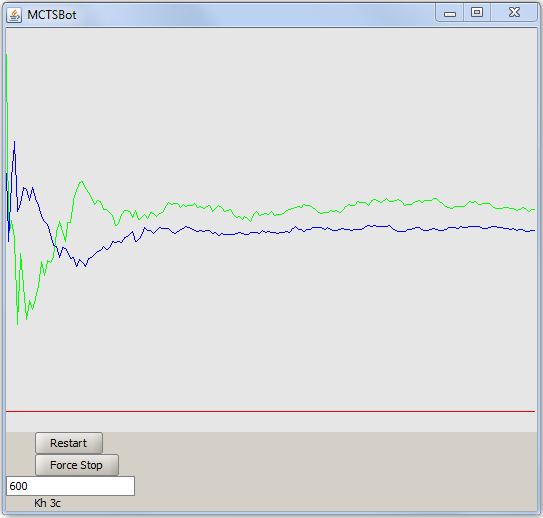
\includegraphics[width=144mm]{Screenshots/GUI.png}
\caption{A GUI for viewing up to date information \\
about the progress of the MCTS algorithm.}
\label{screenshot:gui}
\end{figure}

%TODO: add a screenshot

%So, the GUI was a useful tool in helping me to debug and test the program. It might have been a better idea to implement it earlier in the project than I did (maybe even right at the start) but it still helped me a lot. 



\section{Summary}								% ----

% Review of everything so far.
% Mention the size of the code base. 
% Mention preliminary results.

%Overall, this was a very large project, over 5000 lines of code in total. I'm sure there's probably still a few bugs in it but, as a whole, the program definitely works. From preliminary testing, I have determined that \mbt can usually beat \sbt at a rate of about \$0.20 per game. To put that in perspective, my earliest working version of the program (from Michaelmas term) was losing at about a rate of \$0.25 per game. 

Overall, this was a very large project\footnote{Over 5000 lines of code in total and 58 classes.} and its performance matches my expectations. From preliminary testing, I have determined that \mbt can usually beat \sbt at a rate of about \$0.20 per game. To put that in perspective, my earliest working version of the program (from Michaelmas term) was losing at about a rate of \$0.25 per game. 

In the next chapter, I will evaluate the program much more thoroughly in a variety of situations. 




























\cleardoublepage
\chapter{Evaluation}
% Syntax for images is:
%\begin{figure}[h!]
%\centering
%\includegraphics{}
%\caption{}
%\label{}
%\end{figure}

% Intro											% ----

% What did I want to test?
% Predictions/baseline.


%TODO: update this
In this chapter, I will describe the experiments I performed to evaluate \mbt. There are 4 parameters that I will be altering, they are:
\begin{enumerate}
\item The thinking time available for the MCTS algorithm. 
\item The presence/absence of the two different opponent models. 
\item The selection strategy.
% being used and its parameters.
\item The number of opponents.
%\item The type of the opponent (\sbt or another poker bot).
\end{enumerate}

%In this chapter I will be varying each of these factors to see what effects they have on the performance and play style of \mbt.


\section{Experimental Setup}					% ----

% Producing the graphs and the Exporter class. 
% Why \sbt?
% Default settings?
% Clarify what is meant by performance.
% There are a total of 53488 games played by \sbt.

% TODO: write a brief intro, talk about the default values used and my machine specs.

%Before I get started with the evaluation, I will briefly explain the experimental setup that I used.

% Doesn't sound right.
% First, I made the necessary changes in the \mbt source code and exported a new jar file to the location required by \pa. I then started \pa and created a game between \mbt and \sbt (or other opponents if needed). I started the game and let it run overnight. In the morning, I stopped the game and exported the hand histories. Because I had already made a class to convert the hand histories, I used it again to calculate the profit per hand and write that to a file. I then created the graphs using a program called rlplot. Everything was done on the same computer for consistency.\footnote{The specs of the computer are: Quad Core 2.4GHz CPU ; 3GB RAM; running Windows~7. However the program is only single threaded so only one core was being used. I also noticed that the CPU was almost always the limiting factor.}


To perform most of these experiments, I played \mbt against \sbt in \pap and exported the hand histories. Because I had already made a class to convert the hand histories, I used it again to calculate the profit per hand and write it to a file. I created the graphs using a program called rlplot. Everything was done on the same computer for consistency\footnote{The specs of the computer are: Quad Core 2.4GHz CPU ; 3GB RAM; running Windows~7. However the program is only single threaded so only one core was being used. I also noticed that (one core of) the CPU was almost always at maximum utilization and so was probably the limiting factor.}.

Unless specified otherwise, the default parameters were:
\begin{itemize}
\item 600ms thinking time.
\item Both opponent models (using the EverythingWekaFormat, Weka's NaiveBayes classifier and training data from the 50,000 games of \sbt Vs. \sbt).
\item The UCTVar selection strategy (with opponent model and constants \mbox{\(C_1 = 10\)} and \(C_2 = 0.1\)) and the averaging var backpropagation strategy.
\item The always call simulation strategy (with opponent model).
\item A single opponent, \sbt.
\end{itemize}
% Explain why I used these?

I chose these values by trial and error, they are not necessarily optimal.

In these experiments, I will be measuring the average profit. The profit for one game is the difference between the amount of money \mbt has at the start and the amount of money it has at the end. The average profit is the mean of the profits for every game so far. It is measured in small bets per game\footnote{A small bet is the amount a player can raise by in the first two stages of the game (it is equal to \$1 in this case).}. I am measuring the average profit because I believe it provides a good indication of the overall performance of \mbt. 



\section{How Many Games?}						% ----

% Need to know how many hands to be sure that the results are not due to chance. 
% Assume that each hand is independent. Is this valid?
% Assume that each hand is drawn from the same distribution. Is this valid?
% Need to work out how many hands to do before I can say there is a X% probability that it's not due to chance.
% This depends both on the stdev of data and differences in mean between two different sets of data. 


There are many random elements when playing \sbt against \mbt. The main one being that random cards are dealt to each player and to the table. Also, in \sbt, random numbers are used frequently to decide which actions to take\footnote{In preflop, \sbt has a 5\% chance to play any hand, even if it would have normally folded. In postflop, random numbers are generated and compared to calculated values representing the hand's strength, the pot odds and other values.} and in \mbt, there are several random elements in both the simulation and selection strategies.

%The idea is that over time, the algorithm will reach a stable result. However there are still likely to be a few occasions where random chance effects the final decision. 

I needed to find out approximately how many games it is necessary to play in order to reach a stable result\footnote{If I had had more time then I would have investigated using statistical hypothesis testing~\cite{hypothesis}.}.

%Because of this, I cannot play out too few games and then risk drawing false conclusions from the results. However, it would be pointless and time consuming to play out millions and millions of games if only a few thousand were needed. I need some kind of middle ground.

%In my original proposal, I said that I thought around one thousand games would be sufficient. From preliminary testing, I know that this is not correct. In my progress report, I said that I thought around ten thousand games would be sufficient. 
%I am currently predicting that that is correct and it will require around ten thousand games. 
%I think that this is more accurate and it will require around ten thousand games to reach a stable result.

%Of course, I still haven't said what I will actually be testing for and the number of games required to be able to reach a conclusion will vary depending on that. For example, if I wanted to determine whether using an opponent model will increased performance relative to not using an opponent model, I might only need to play a few thousand games because I would expect there to be a very large difference in performance. However, if I wanted to determine if there was an increase in performance by increasing the thinking time from 600ms to 700ms, I would probably have to play hundreds of thousands of games because I would expect the increase in performance to be small. 

To get a rough idea of how many games are necessary, I played out almost 65,000 games of \sbt Vs. \mbt using the default parameters. Here is a graph of \mbts average profit over the course of those 65,000 games. Note that the dotted lines are drawn at two times the standard error from the mean. 
% This means that I can say there is a 95\% that the 
% Why?
\begin{figure}[H]
\centering
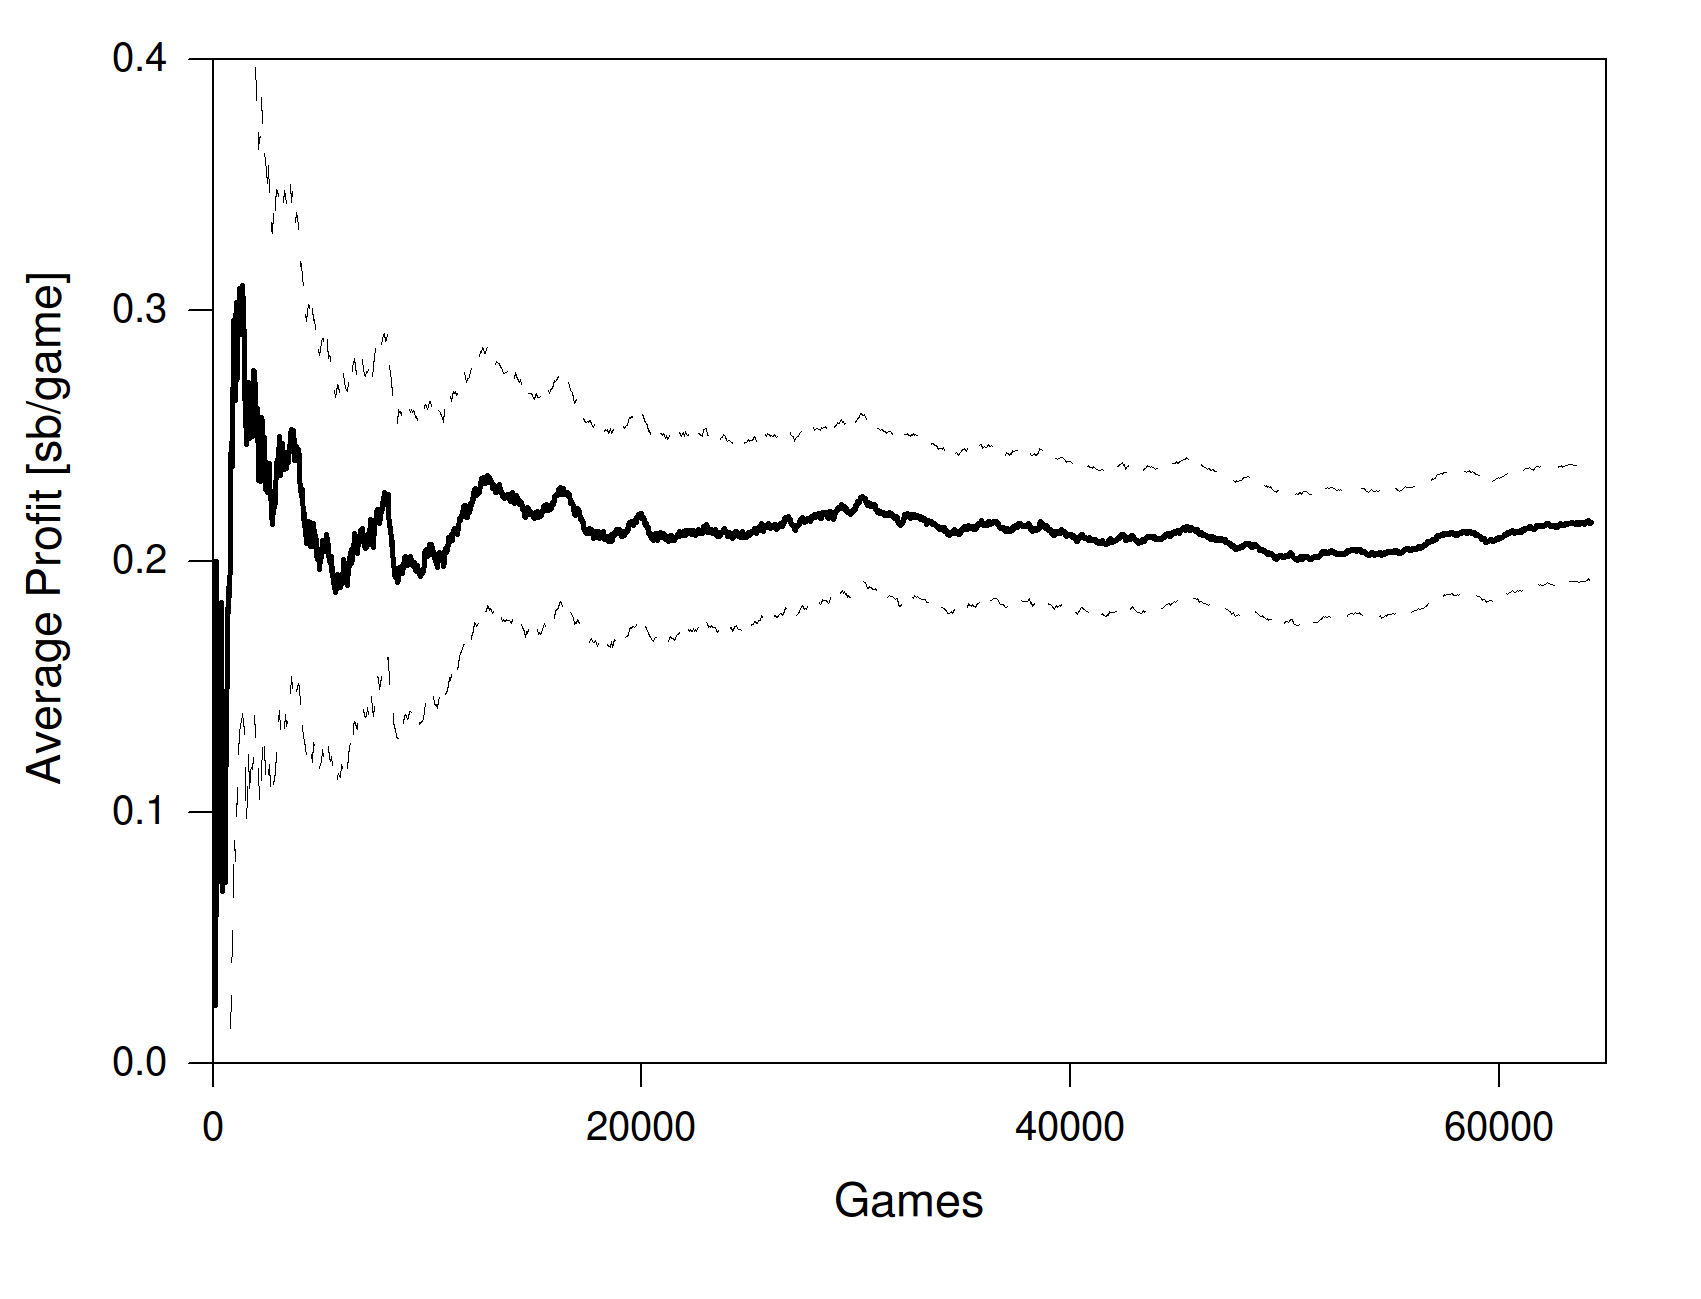
\includegraphics[width=144mm]{Graphs/SBvMB-600-65k-v2.png}
\caption{\mbt Vs. \sbt{} - 65,000 games with default parameters.}
\end{figure}

%From looking at this graph, there doesn't appear to be a whole lot of change after about the 20,000 mark. 
%It's also worth noting the scale on the left, 
%Based on this, I plan to play out 20,000 games (for each variant) in the following experiments. However I may do less if it becomes obvious that it is not needed.

There seems to be little change after 20,000 games. Based on this, I planned to play out 20,000 games (for each variant) in the following experiments\footnote{Again, if I had more time then I would take a much more thorough approach. However, it can take over 24 hours to play out 20,000 games and so playing more is simply not practical.}.



\section{Varying Thinking Time}					% ----

% Want to see if there is a difference.
% Want to see how much of a difference there is. 
% Want to see if there is a simple model to describe the profit as a function of thinking time. 
% How much was I varying thinking time by?
% What was I not varying?
% My predictions?


%From the literature on MCTS and from my experience so far, I expect the performance to increase as thinking time increases. What I don't know is how much the performance will increase by. I doubt it would be a simple relationship since the program is incredibly complex. 

%I predict that, at very high thinking times, the performance will level out to a constant-ish value. I think this because no matter how good \mbts decisions are, its profit is still limited by the rules of poker and by \sbts play style. I also think that the performance will not decrease as the thinking time increases. I think this because the MCTS algorithm is relatively stable and should always reach a point where its answer will not change. At very low thinking times, I'm not sure exactly what will happen. I think there could be a point where \mbt starts to lose to \sbt but I don't know when that will be.

From the literature on MCTS and from my experience so far, I expected the average profit to increase as thinking time increases. I also expected the average profit to eventually level out. This is because no matter how good \mbts decisions are, its profit is still limited by the rules of poker and by \sbts play style. 

To test the effects of thinking time on performance, I ran five trials of 20,000 games each. The only variable I changed was the amount of thinking time given to the MCTS algorithm. 
%I will use the default thinking time, 600ms, as well as 2400ms, 150ms, 38ms and 9ms. I have chosen these values because I think they represent a wide range of abilities for the MCTS algorithm. 
I used the default thinking time (600ms) as well as four times the default (2400ms), one quarter of the default (150ms), one sixteenth of the default (38ms) and one sixty fourth of the default (9ms). I chose those values because I think they represent a wide range of abilities for the MCTS algorithm. 

Here is a graph showing the average profit for the five different thinking times. The error bars are drawn at two times the standard error from the mean. Also note that time is on a log scale.
\begin{figure}[H]
\centering
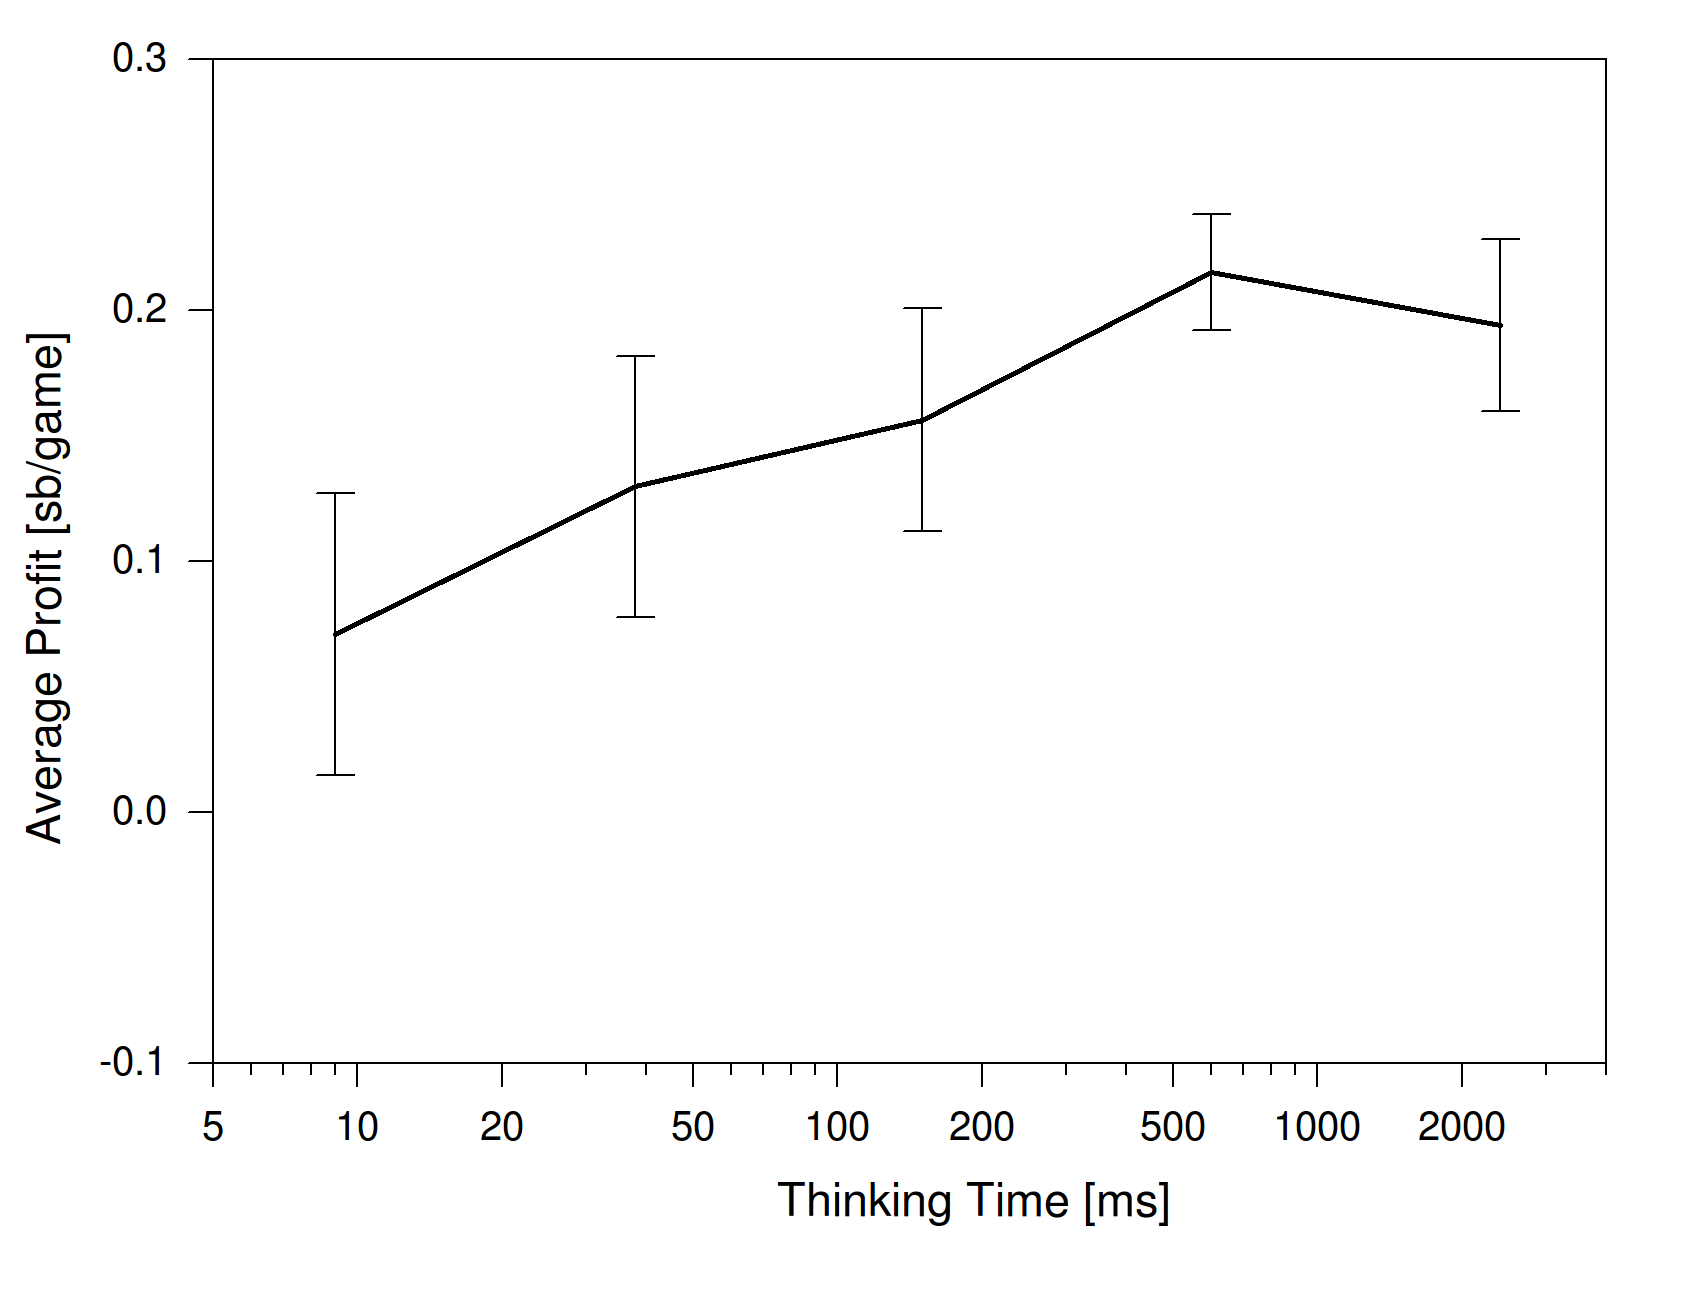
\includegraphics[width=144mm]{Graphs/SBvMB-time.png}
\caption{Average profit of \mbt against \sbt \\ with different thinking times.}
%\label{}
\end{figure}

%From these results, I think it clear that the thinking time does in fact have a significant effect on the average profit. 

I think it is clear from these results that increasing the thinking time has a positive effect on the average profit. 

At 2400ms thinking time, the average profit is slightly lower than at 600ms. Given that both means lie within the error bars of the other, it is most likely due to chance\footnote{However, it could also be caused by something else. If I had more time, I would investigate this further.}. 





\section{Varying Opponent Models}				% ----

One of the original questions I wanted to answer was: how much of an effect do the opponent models have? To find out, I played \mbt against \sbt using all four combinations of the two opponent models, that is: both of them, just the hand rank opponent model, just the next move opponent model and neither of them. 

Note that when I say an opponent model is not being used, I mean that I am using the basic model instead of the one using Weka classifiers. The basic hand rank opponent model is the one which randomly deals the opponent some hole cards and sees who has the best hand. The basic next move opponent model is the one which assigns a probability of \(1 \over 3\) to each of the possible moves\footnote{A basic model which returned different probabilities might perform slightly better. I did briefly experiment with using different probabilities, however it still did not perform very well.}.
%was still no where near as good as the opponent model using Weka.}.
%I obviously expect the trial using both opponent models to do best. I also think that the the trial using only the next move model will do better than the one using only the hand rank opponent model. I think this because 


%Here is a bar chart displaying the average profit with the four different combinations of opponent models.
Here is a bar chart displaying the results, the error bars are drawn at two times the standard error from the mean\footnote{Note that the no-models and hrom-only results were attained after only 5000 games. This was due to time constraints.}.
\begin{figure}[H]
\centering
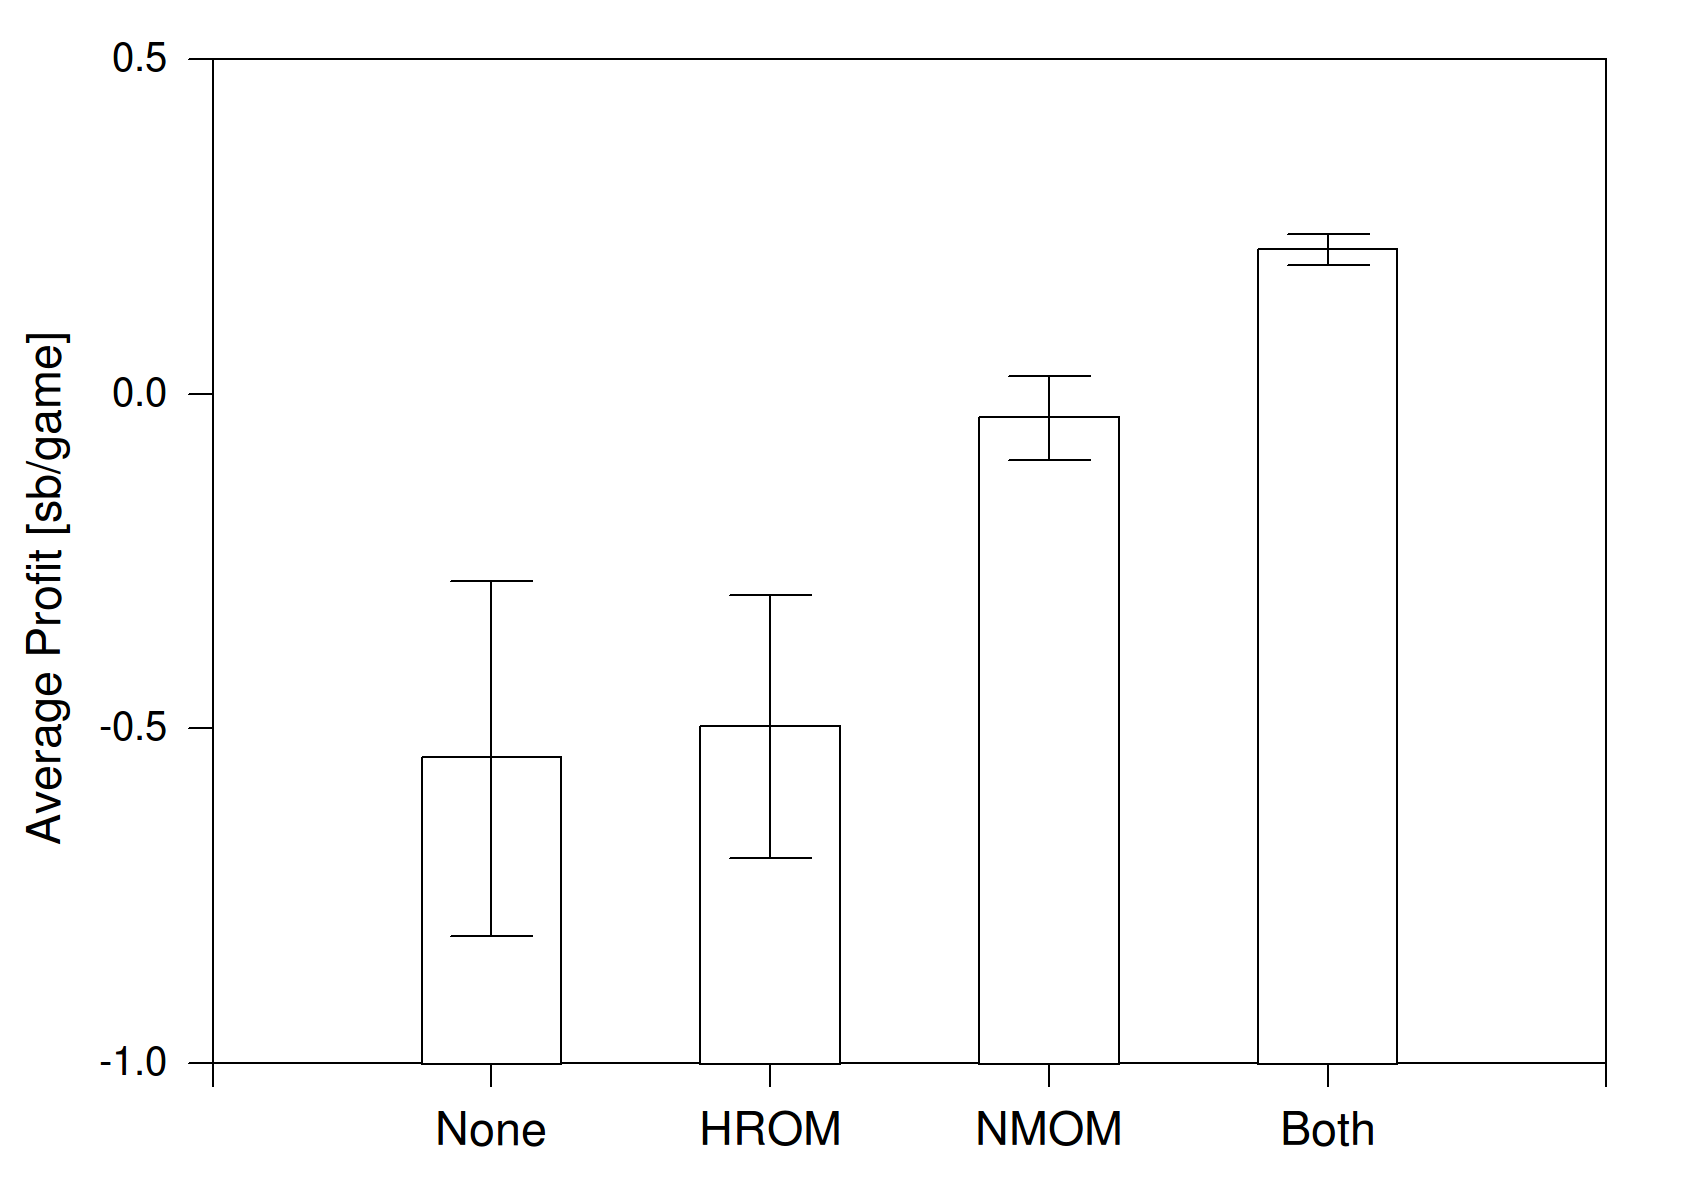
\includegraphics[width=144mm]{Graphs/SBvMB-oppmodels-v2.png}
\caption{Average profit of \mbt against \sbt \\ with different combinations of opponent models.}
%\label{}
\end{figure}

The graph shows that using both opponent models is far superior to any other combination. In fact it is the only combination which actually makes a positive average profit.
%Using only the next move opponent model produces a much higher average profit than using only the hand rank opponent model or no opponent models. 
Using only the next move opponent model is the next best, almost managing to break even. The other two combinations both perform equally poorly.


I think these results show that both opponent models clearly benefit the program and that the next move opponent model is more beneficial than the hand rank opponent model.
%\footnote{Which is consistent with my expectations.}. 





\section{Varying Selection Strategies}			% ----

When dealing with \choices, there are two possible selection strategies, UCT and UCTVar. 
%From early testing, I remember the UCTVar strategy giving a slight increase in performance. 
%I predict that the UCTVar strategy will still do slightly better, although I don't know how much better. 
Here is a bar chart showing the average profit for each strategy. Note that I used \(C = 10\) for the UCT strategy and \(C_1 = 10\) and \(C_2 = 0.1\) for the UCTVar strategy. The error bars are drawn at two times the standard error from the mean.
\begin{figure}[H]
\centering
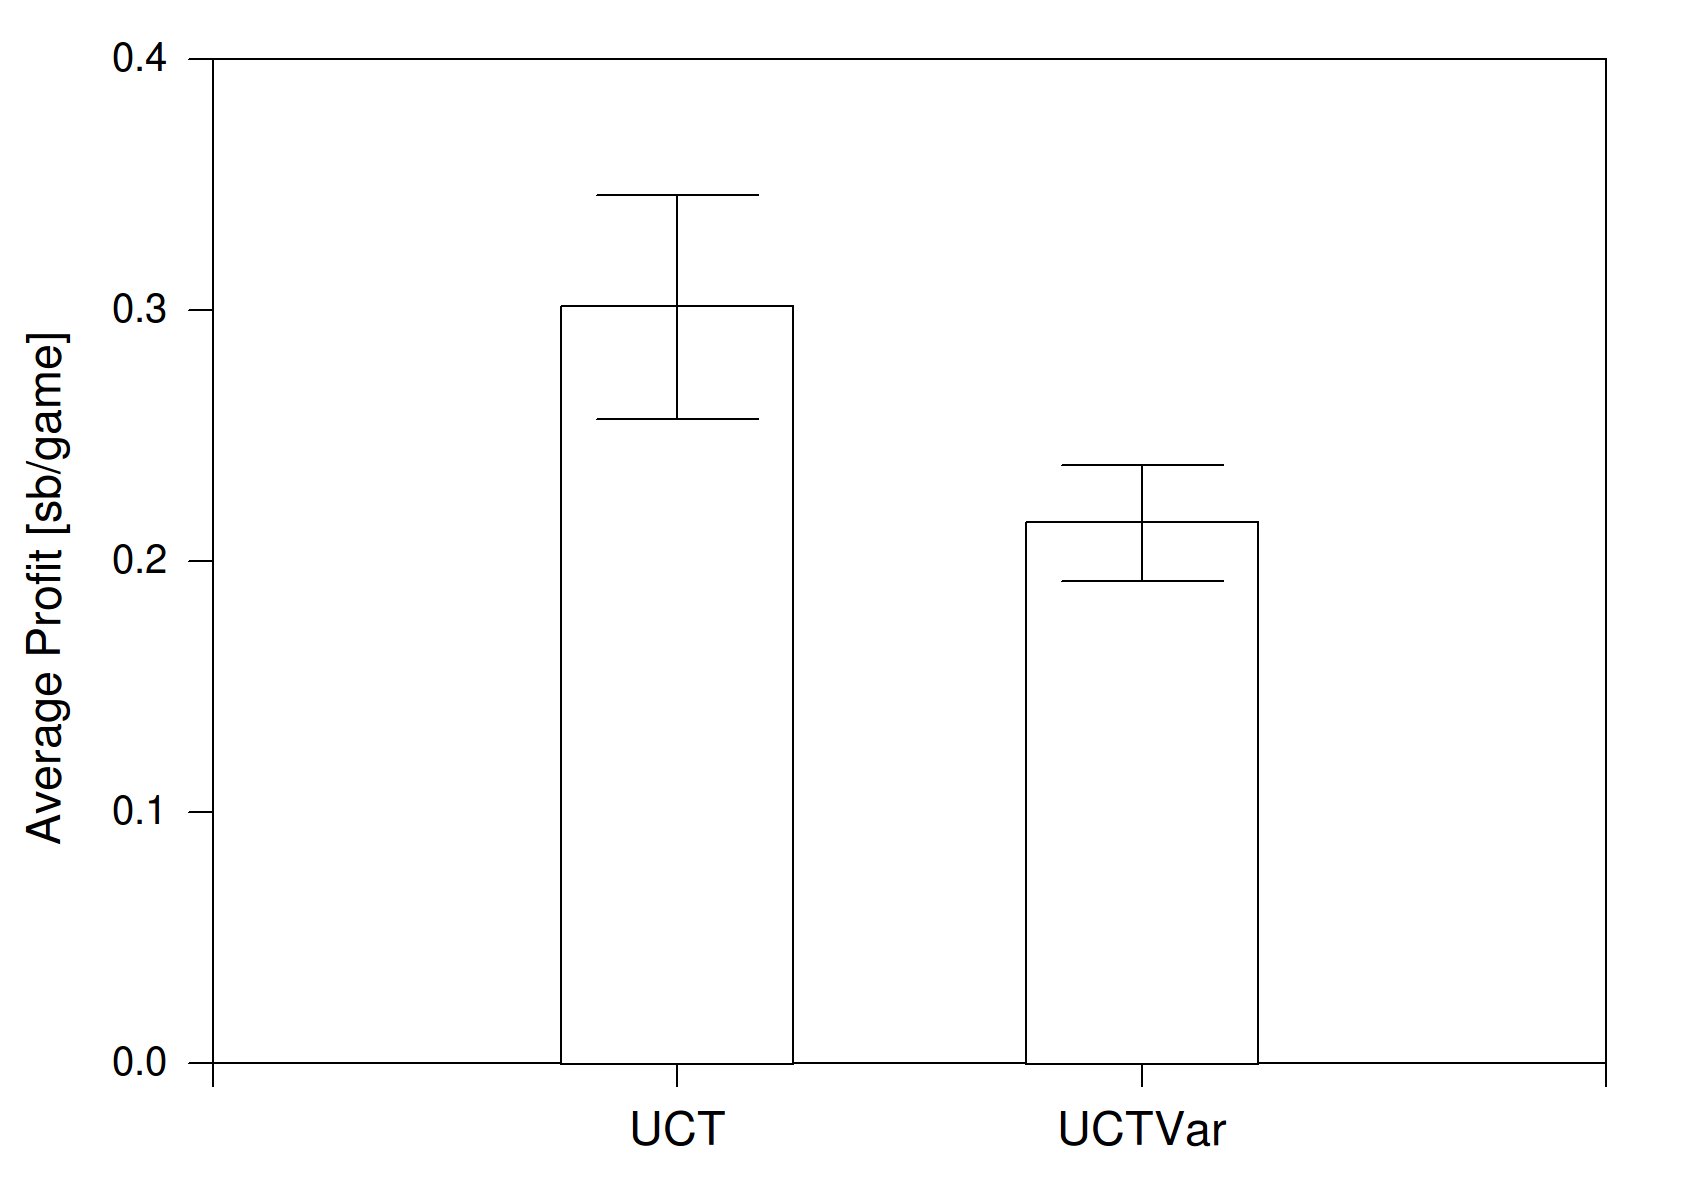
\includegraphics[width=144mm]{Graphs/SBvMB-UCT.png}
\caption{Average profit of \mbt against \sbt \\ with the UCT and UCTVar selection strategies.}
%\label{}
\end{figure}

The results clearly show that the UCT strategy is performing significantly better than the UCTVar strategy. This is exactly the opposite of what I expected\footnote{I am not sure how to explain this, especially as I remember the UCTVar strategy performing better in early testing. I think I might have inadvertently fixed a crippling bug in between testing the two strategies, which made me think that the UCTVar strategy was increasing the performance.}.

The reason for this might be that I am not using the best possible constants. I may also have implemented the UCTVar strategy incorrectly or there could be bugs in the code. All I can say is that, in my implementation, the UCT strategy is superior to the UCTVar strategy.



\section{Varying the Number of Opponents}		% ----

Another one of the original questions that I wanted to answer was: what effect does increasing the number of opponents have? 
%In this section I will try to answer that question. 
There are several things to consider.
%when increasing the number of opponents. 
The first is that, when there are more opponents, there is a lower probability that \mbt will have the best hand\footnote{In fact you would expect the probability to be \(1 \over n\) where \(n\) is the total number of players in the game.}. The second is that the MCTS algorithm does not explicitly take into account the fact that when an opponent does stay in the game, they are more likely to have a better hand than if they had made the same actions in a game with fewer players. This is because the opponent model was trained on data from two player games only. Also, since there are more players in the game, there will be a greater number of branches in the game tree and so the MCTS algorithm will have less time to search through each one. 

On the other hand, you could argue that \mbt has more opportunities to win money through superior play. However, I was still expecting \mbts average profit to decrease as the number of opponents increases. 

The following graph shows the average profit of \mbt when played against one, two, three and four separate instances of \sbt in \pap. Error bars are drawn at two times the standard error from the mean.
\begin{figure}[H]
\centering
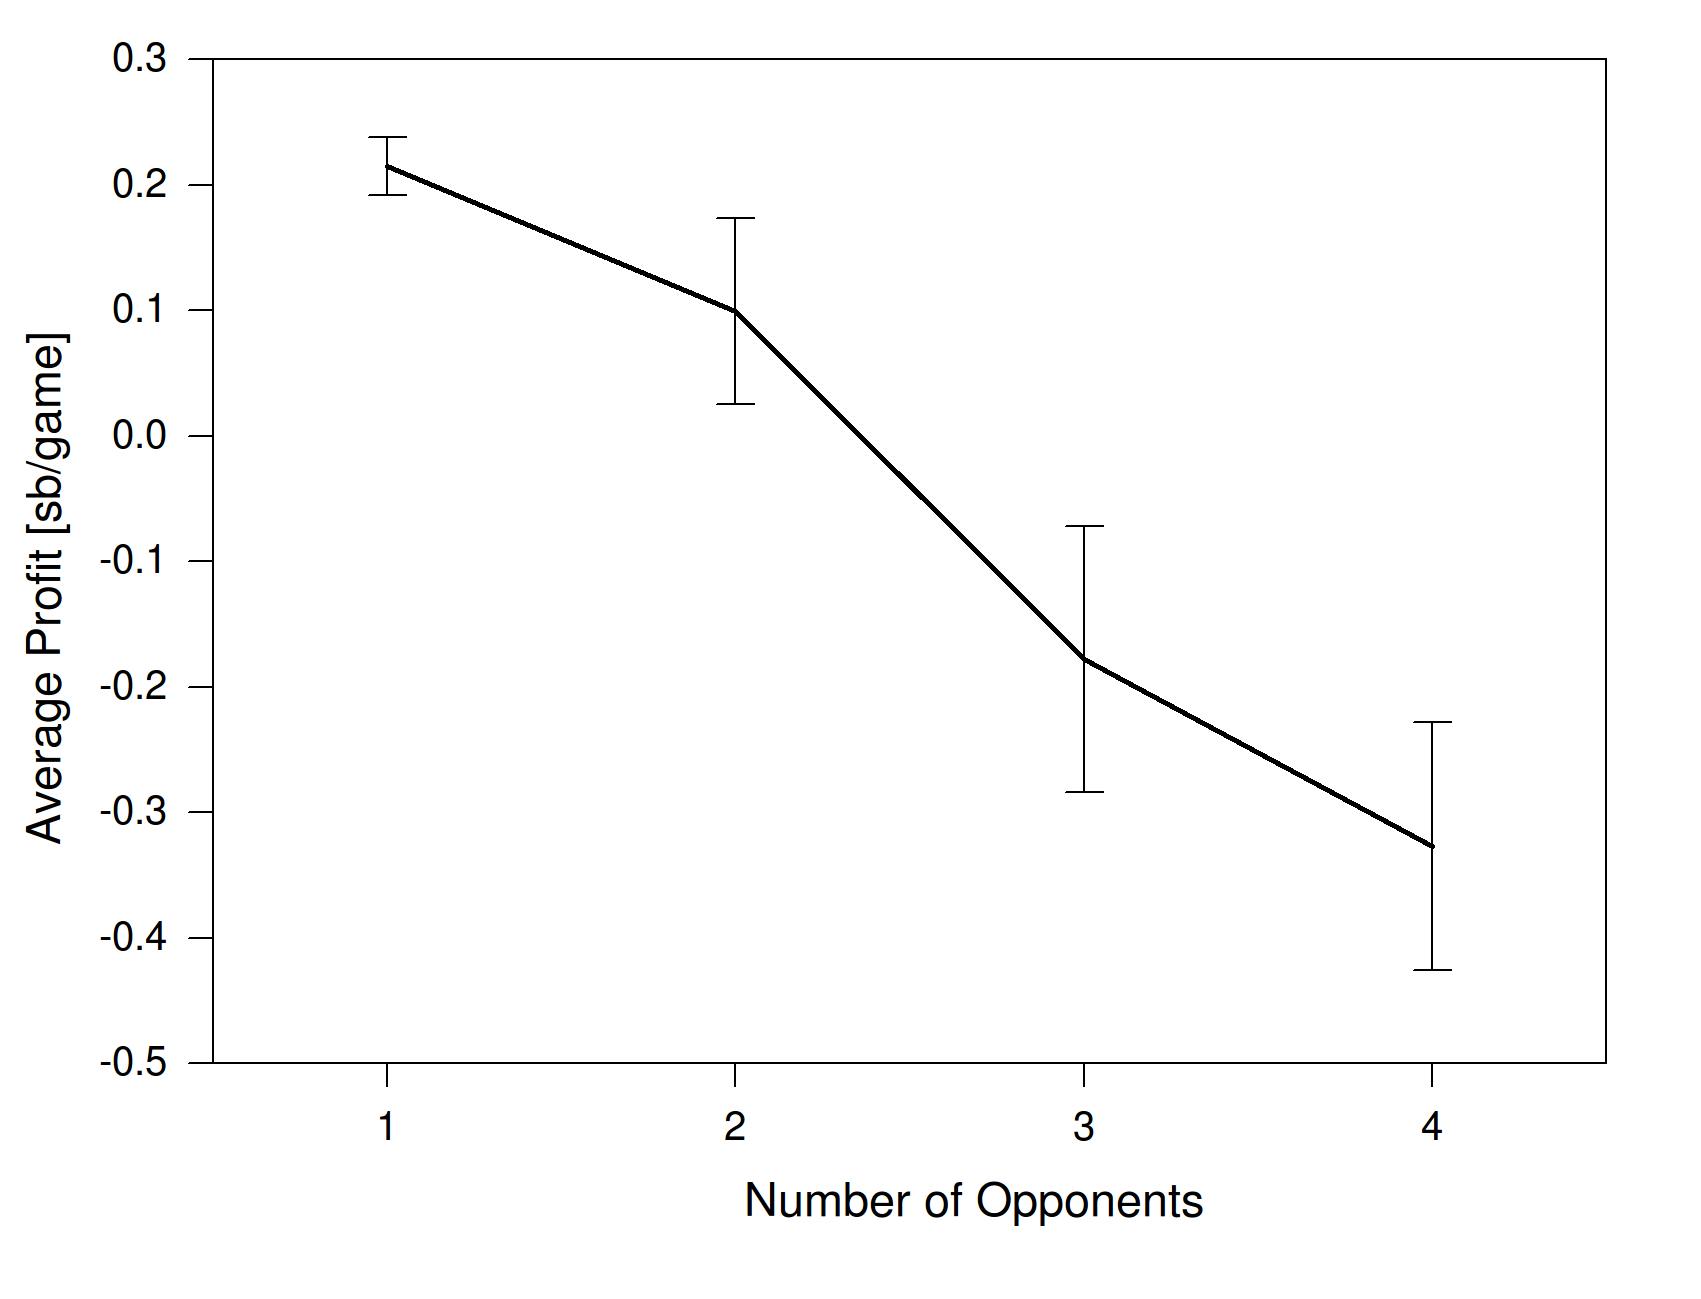
\includegraphics[width=144mm]{Graphs/SBvMB-num.png}
\caption{Average profit of \mbt \\ when played against multiple instances of \sbt.}
%\label{}
\end{figure}

As you can see, the average profit steeply decreases as the number of opponents increases. \mbt is able to make a positive average profit when played against one or two opponents but not when played against three of four. 
%This is consistent with my expectations. 




One of my original success criteria was for \mbt to be able to make the most money when played against three separate instances of \sbt. In the above experiment, \mbt did not achieve this. However, I now know that the default settings I have been using are not optimal. I wanted to complete all of my original success criteria so I attempted to tweak the parameters of \mbt to increase its performance. 

I decided to use the UCT selection strategy (with \(C = 10\)) instead of the UCTVar selection strategy. I also gave the MCTS algorithm 1000ms thinking time instead of 600ms. The following graph shows the average profit of \mbt and all three of the instances of \sbt.
\begin{figure}[H]
\centering
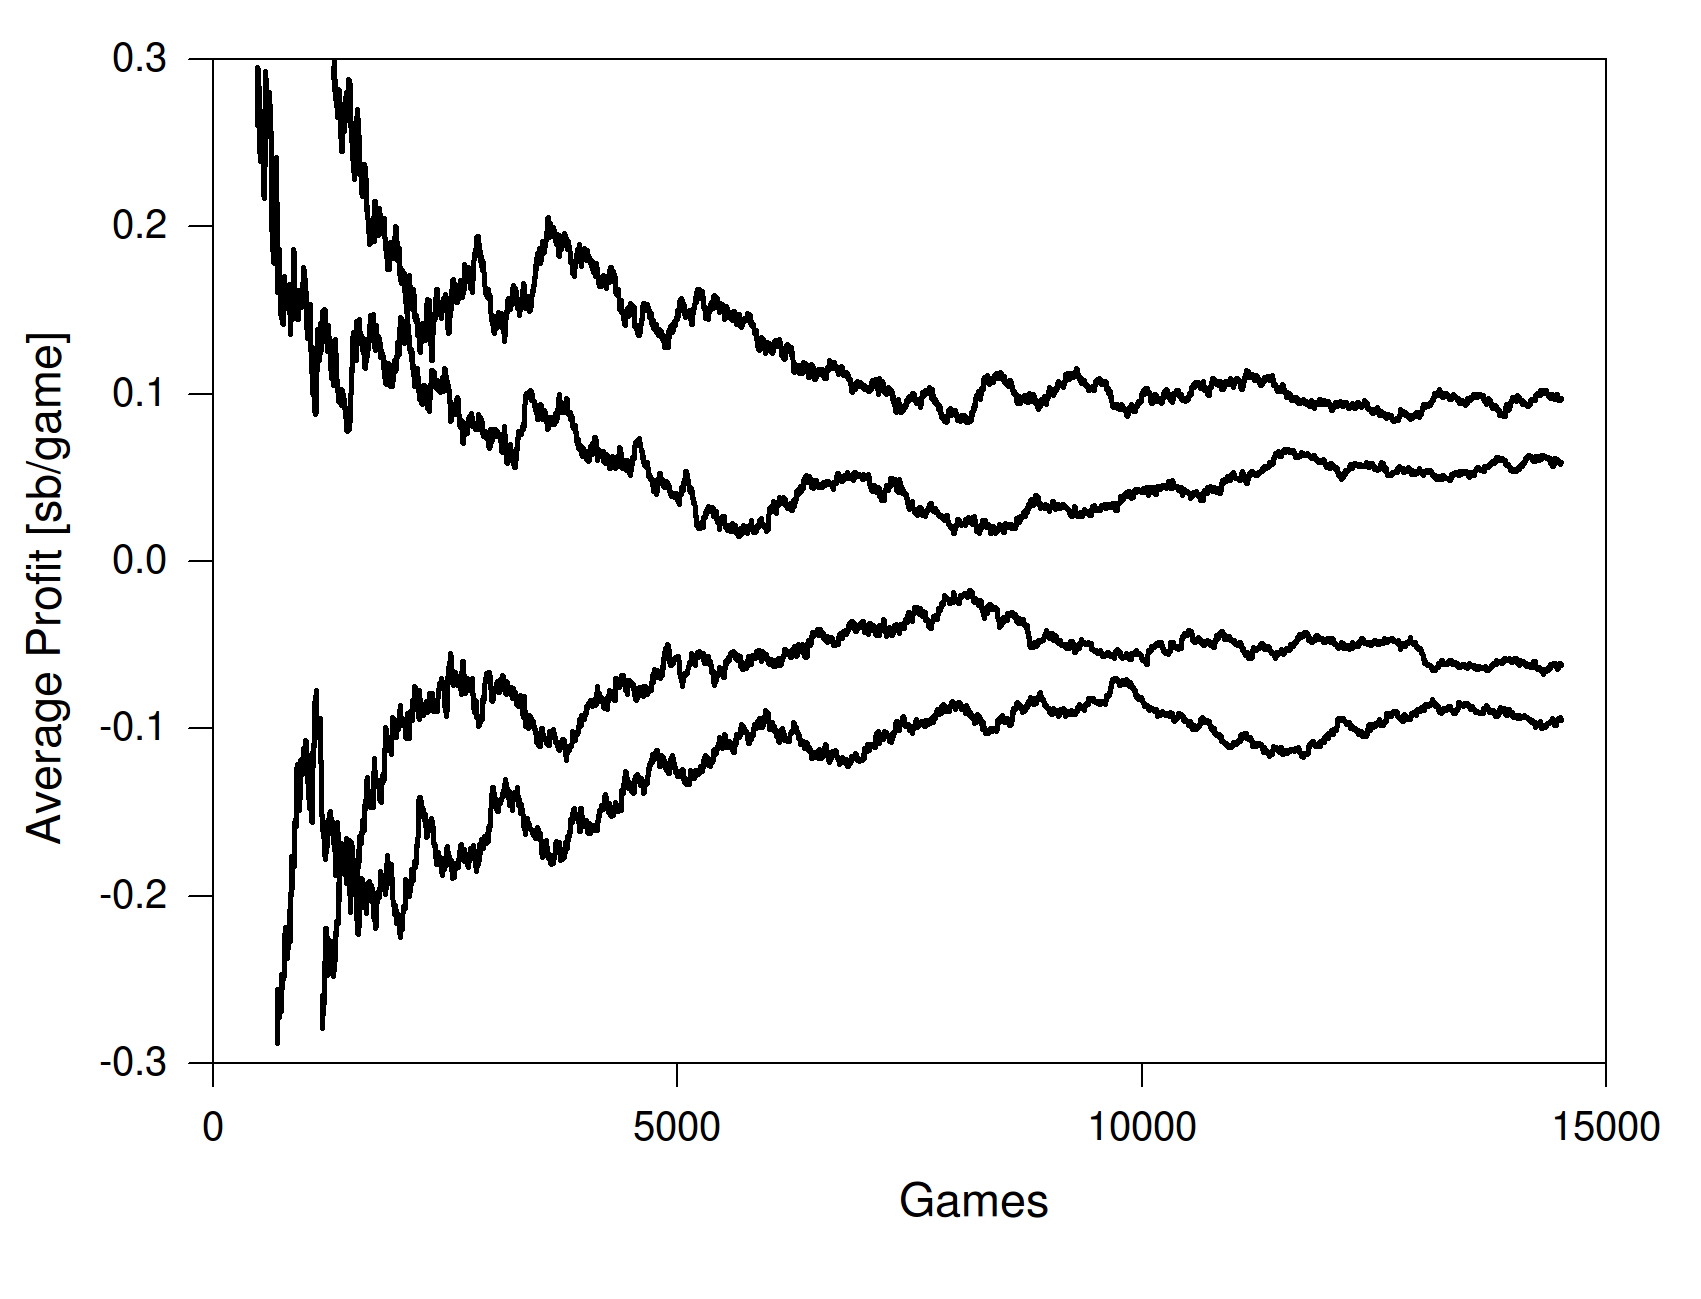
\includegraphics[width=144mm]{Graphs/SBvMB-x3.png}
\caption{Average profit of \mbt and three instances of \sbt \\ over the course of about 15,000 games.}
%\label{}
\end{figure}

The top line is \mbts average profit, 
%the line below that is \sbt{}3's average profit, the line below that is \sbt{}2's average profit and the bottom line is \sbt{}1's average profit. 
the three lines below that are the average profits of the three instances of \sbt\footnote{In my opinion, this shows that \mbt can make the most money when played against three instances of \sbt. If I had more time, I would play more games and try to show this more conclusively.}.

An interesting thing to note is that the \sbt which was sitting to the right of \mbt, seems to be doing much better than the other two instances of \sbt. I have noticed this every time I have played games with multiple opponents. I think this could be due to a situation in which \mbt has a bad hand but gets drawn into the next round with the player to its right just because it is on the big blind.

% Add footnote saying if I had more time...



\section{Other Opponents}						% ----

I originally chose \sbt because it was simple yet still challenging. However, I think it would be interesting to see how my program fares against some other poker bots. 
%In this section, I will play \mbt against some of the other poker bots included with \pap.

Here is a table showing the average profit of \mbt when played against the opponents included in \pap{}\footnote{Note that due to time constraints, I was only able to play about 3000 games for each opponent.}.
\begin{center}
\begin{tabular}{c|c}
Opponent & Average Profit \\
\hline
%\sbt & +0.21 sb/game \\
Simbot & +0.39 sb/game \\
Jagbot & +0.22 sb/game \\
Pokibot & -0.75 sb/game \\
Sparbot & -0.75 sb/game \\
Vexbot & -1.75 sb/game \\
\end{tabular}
\end{center}

\mbt appears to perform well against Simbot and Jagbot, poorly against Pokibot and Sparbot and extremely poorly against Vexbot. I think this shows that, when designing a poker bot, it is important to test against a wide variety of opponents because some strategies may be effective against some opponents and ineffective against others.



Note that \mbt is using the default parameters, including the opponent models trained on the \sbt Vs. \sbt hand histories. This means that a lot of \mbts strategy is specific to \sbt. I have observed that Vexbot in particular seems to exhibit behaviours which \sbt does not. For example, sustained attempts at bluffing. I think that if I were to implement a more general opponent model, it would increase \mbts playing ability when facing other opponents.



%As you can see, \mbt isn't doing too well. I think this is mostly due to the fact that it is still using the opponent models trained on the \sbt Vs. \sbt hand histories. I have observed that Vexbot in particular seems to exhibit behaviours which \sbt does not. For example, sustained attempts at bluffing. 

% Add this to the conclusion
%I think that, if I had more time, I might be able to tweak \mbt to perform better. I also think that I could create a more general opponent model, capable of more accurately predicting the actions of other opponents and maybe even adapting to different opponents on the fly. Alas, I do not have time to complete any of those extensions.




%\section{Profit Distribution}					% ****

%TODO


%\section{General Notes on \mbts Play Style}		% ****

%In this section, I will briefly give some of my thoughts about \mbts play style when facing \sbt. 

%TODO: or put in the conclusion?




%\section{Summary}								% ****


%TODO: or don't bother and just do it in the conclusion




\cleardoublepage
\chapter{Conclusion}
\section{Results}

My program, \mbt, has proven to be a competent poker player when facing simple opponents. It can consistently beat \sbt in a two player match. It can also beat three separate instances of \sbt in a four player match.

I have also demonstrated the effects on performance of varying factors such as the thinking time, the presence of the opponent models, the selection strategy and the number of opponents. 

%I am very pleased with these results and with the success of the project as a whole.



\section{Future Work}

I think the biggest weaknesses of \mbt are its limited opponent models. Currently, they are too specific to \sbt and too specific to games with only two players. This means that \mbt will often make poor choices when facing other opponents or playing in games with more than two players. 

I would like to expand the opponent models for use against other opponents. I also think it would be interesting to create an opponent model with the ability to adapt to unknown opponents or maybe one which could learn from its own mistakes. 

%I also think that the way in which I implemented the opponent models is not particularly elegant. Given more time 

%I also think that there is potential to improve the simulation strategy. 



\section{Summary}

% summary of whole project
% stuck to plan?
% errors made

In this project, I have successfully built a working poker bot. I implemented the \mcts algorithm with several alternative strategies and I created two simple opponent models. 

%I stuck to my original plan quite closely although it took a lot longer than I had anticipated. If I had to restart this project, I would do two things differently. First, I would use opentestbed instead of \pa. \pa is not ideal for evaluating poker bots and it provides no way to control the random elements in poker. Second, I would approach the opponent models in a different way. I think that my current design is a little too difficult to maintain; making simple changes can sometimes require several different files to be edited.

I stuck to my original plan quite closely although it took a lot longer than I had anticipated. If I could go back and change one thing, I would have chosen opentestbed instead of \pa. \pa is not ideal for evaluating poker bots and it does not provide a way to control the random elements in poker.


However, I am delighted with the results I have achieved and with the success of the project as a whole.










%%%%%%%%%%%%%%%%%%%%%%%%%%%%%%%%%%%%%%%%%%%%%%%%%%%%%%%%%%%%%%
% The Bibliography

\cleardoublepage
\chapter*{Bibliography}
\addcontentsline{toc}{chapter}{Bibliography}
\bibliographystyle{plain}
\bibliography{refs}
\cleardoublepage


%%%%%%%%%%%%%%%%%%%%%%%%%%%%%%%%%%%%%%%%%%%%%%%%%%%%%%%%%%%%%%
% The Appendices
\appendix

%\chapter{The Rules of \texasp}
%\hypertarget{rulesoftexas}{}
%\label{app:texrules}
%TODO: just copy and cite the wiki page?


%\cleardoublepage

%\chapter{\sbt Source Code}
%\hypertarget{simplebotsourcecode}{}
%\label{app:sbsource}
%\input{simplebotsource}

\cleardoublepage

\chapter{Project Proposal}
\begin{flushright}
David Moody			\\
Christ's College	\\
dm484				\\
\end{flushright}

\vspace{16pt}

\begin{center}
{\large Diploma in Computer Science Project Proposal}		\\
\vspace{4pt}
{\bf \huge Monte Carlo Tree Search in \\ 
\vspace{6pt} \texasp}\\
\vspace{12pt}
{\large 17 October 2010}									\\
\end{center}

\vspace{36pt}

\begin{flushleft}
{\bf Project Originator:} Sean Holden\\
\vspace{12pt}
{\bf Resources Required:} See attached Project Resource Form\\
\vspace{12pt}
{\bf Project Supervisor:} Sean Holden\\
\vspace{12pt}
{\bf Director of Studies:} Marcelo Fiore\\
\vspace{12pt}
{\bf Overseers:} Andy Rice and Jean Bacon\\
\end{flushleft}

\newpage


\section*{Introduction and Description of the Work}

There are two types of poker playing program. The first type attempts to approximate a perfect strategy using game theory. While this might be the best way to play if your opponents are also playing with an optimal strategy, it can't exploit the possible weaknesses of your opponents. The second type of  program can exploit the weaknesses in its opponents' strategies. It does this in order to try and maximize its total income and thus outperform the first type. In my project I will be looking at the second type of program.

In the specific variety of poker which I will be using, \texas, each player is first dealt two cards which only they can see. There is then a round of betting in which each player in turn is given the choice to either: raise, where they place an amount of money into a shared "pot"; call, in which case they must put into the pot the same amount of money as the last person in the current round who raised (possibly nothing); or fold, in which case they forfeit the game and lose any chance to win the money in the pot. After this round of betting, three shared cards are dealt which everyone can see. Then there is another round of betting, another shared card, another round of betting, another shared card and a final round of betting. At this point, it more than one player is still in the game then the player who can make the best ``poker hand'' out of their cards and the shared cards wins the money in the pot. If all but one player folded before this point then the remaining player wins the money in the pot.

There are two main varieties of \texas. In the first (no-limit), you can raise any amount that you want. In the second (limit), you can only raise by a fixed amount. While no-limit \texas might also make a good game for this project, I will be using the limit variety.

Poker is usually played with somewhere between 2 to 10 players. When you have only 2 or 3 different players it is feasible to do a complete search of the game tree in order to find an estimate of what you think the optimal strategy would be. However, when you are playing with more than 3 players the game tree becomes much much larger. In a game with 10 players it would be impossible to do a complete search of the tree. 


Thus we need to use an algorithm that can approximate the best choice without needing to search the whole tree. Monte Carlo Tree Search can do this by randomly simulating many games and using the results of those simulations to construct a partial game tree with estimates for the expected values of the nodes.

The MCTS algorithm consists of 4 main stages:

\begin{enumerate}
\item Selection: In this stage, starting at the root, you need to select which branch of the tree you want to explore further. I will be investigating multiple selection strategies including random selection, Upper Confidence Bound selection and selection using a complex opponent model to predict your opponent's most likely action.
\item Expansion: Once you reach a leaf in the stored partial tree you need to expand the tree by adding new nodes. You simply need to decide if the node of the partial tree is also a node of the full game tree and if not you need to add children representing the possible actions that could occur next.
\item Simulation: Starting from one of the newly added children, you need to simulate the completion of the game. There are several ways in which you could do this including random simulation or simulation based on more complex heuristics. I will investigate multiple simulation strategies. Once you have simulated the game to completion you need to calculate the expected value of the game state. The opponent model will be used to attempt to estimate what the opponents' cards may be based on their previous actions, thus allowing you to estimate the expected value of the game state.
\item Backpropagation: Once you know the expected value of the simulated game, you need to update the expected values of the nodes in the path that you took to include this information.
\end{enumerate}

These 4 steps are repeated to build up the game tree until there is no more time left for computation. An action is then chosen, usually based on the highest expected value of the children of the root node. 


In order to take advantage in the weaknesses in our opponents' strategies we also need an opponent model capable of predicting the following two things:

\begin{enumerate}
\item The probability that an opponent will perform a specific action given their actions up to this point in the game and the shared cards currently on the table.
\item The probability that an opponent has specific cards in their hand given their actions throughout the current game and the 5 shared cards on the table.
\end{enumerate}

I will use Weka's \cite{propweka} algorithms to create regression models for each of these.

Training data for the first model will be take the following form: \\*
\(A_1, C_1, C_2, C_3, A_2, C_4, A_3, C_5, A_4\) \\
Where \(A_i\) is the action (fold, call or raise) taken by the opponent at step i and \(C_j\) is the \(j_{th}\) shared card to be dealt. I may experiment with different ways of representing the cards.

I think I would need to have separate regression models for predicting each \(A_i\). i.e. the training data for each \(A_i\) would look like this: \\
\(A_1, C_1, C_2, C_3, A_2, C_4, A_3, C_5, A_4\) \\*
\(A_1, C_1, C_2, C_3, A_2, C_4, A_3\) \\*
\(A_1, C_1, C_2, C_3, A_2\) \\*
\(A_1\) 

This would make predicting the first action rather trivial, however it might also be a rather poor way to predict the first action. I might investigate how including other fields, such as the number of players to the right and to the left of the opponent or the position of the player who first raised, affects the ability to predict the first action of an opponent.

For predicting what hand the opponent might have we could use training data of this form: \\
\(A_1, C_1, C_2, C_3, A_2, C_4, A_3, C_5, A_4, H_1, H_2\) \\
Where \(H_1\) and \(H_2\) are the cards held by the opponent.


This also raises the question of where I will get the records of played games (aka hand histories) from which I can extract this training data. There is 70GB of obfuscated (names of players have been changed) hand histories available at source \cite{prophh} which I think will be sufficient and I may be able to find more if required.

Unfortunately this data is not in a form that will be readable by Weka so I will need to write tools able to convert it into the Attribute-Relation File Format which Weka uses.

It will be possible to create training data for the first type of model from every action which takes place in the games. However for the model which predicts which cards the opponent holds, only games in which two or more players remained after the final round of betting can be used.


Once I have a program capable of playing poker I will need to test it to see how well it can play against other poker bots. I will integrate my program with the Poker Academy Pro software and test it against the poker bots which come with the software. I will consider the project a success if it is able to consistently beat a program called SimpleBot \cite{propsb} which only considers its own hand when determining how to play. I will also be testing my program against the other poker bots available with the software, however being able to beat them will not be one of my success criteria because I don't want to be directly competing with the creators of the other poker bots. (Many of the existing poker bots were created by teams of researchers with much more experience than me.)

In addition to testing my program against other programs, I can test different versions of my program against each other to investigate how effective different selection strategies/opponent models are.


For extensions of the project, if I have time remaining after implementing what I have so far described, I would like to look at improving the selection and simulation strategies of the MCTS algorithm and improving the prediction capabilities of the regression models. If I still have time after that I will look at the possibility of changing the opponent model to be able to record statistics about specific players it has played against and alter its decisions based on those observations.


\section*{Resources Required}

\begin{itemize}
\item Algorithms from the Weka toolbox (a free collection of algorithms under the GNU General Public License) \cite{propweka}.
\item Records of online poker games (aka hand histories) available online for free \cite{prophh}.
\item Poker Academy Pro and the Meerkat API for interaction with other poker bots \cite{proppa}. Poker Academy Pro is not free but I don't mind paying the \$85 required to purchase it. The software is only needed when testing the program against other poker bots so it won't be needed to understand or test the majority of the project.
\item The core Java packages and the eclipse IDE.
\item The use of my own computer.
\end{itemize}


\section*{Starting Point}

I already play \texasp regularly and I think I'm familiar enough with the game to be attempting this project.

The Artificial Intelligence I course from part IB contains information about best-first search techniques and machine learning techniques which will be very useful throughout the project.

The Java courses and Algorithms courses from part IA and IB will also be helpful.


\section*{Substance and Structure of the Project}

The aim of this project is to create a poker playing program capable of playing Limit \texas in games with more than 3 players. The program will use Monte Carlo Tree Search to partially explore the game tree and machine learning techniques to create an opponent model capable of predicting the probabilities of an opponents next action. The program will be integrated with the Meerkat API which will allow it to play against other poker bots included with the Poker Academy Pro software.

The project consists of 9 main stages:
\begin{enumerate}
\item Further research into opponent modeling, MCTS and different selection strategies for it, Poker Academy Pro and existing poker playing programs for it, the Weka toolkit, availability/quality of hand histories and how to convert them to ARFF, etc.
\item Creation of the basic framework of the program and integration with the Meerkat API. Also deciding upon how to abstract away some of the unnecessary details in poker.
\item Implementation and testing of the basic MCTS algorithm as described in the Introduction and Description of the Work section.
\item Collection and consolidation of hand histories into Attribute-Relation File Format.
\item Using Weka to create regression models for calculating the required probabilities and integrating those models into the opponent model.
\item Integration of the opponent model with the MCTS algorithm.
\item Evaluation and testing of the program against SimpleBot and other programs using Poker Academy Pro. Investigation into how effective MCTS with an opponent model is when compared to just MCTS. Investigation into the effects of varying the available search time and increasing the number of opponents.
\item Possible extensions such as changing the opponent model to adapt to specific players and trying out and comparing different selection/simulation strategies in the MCTS algorithms. (I don't want to say exactly what I'm going to be doing right now because I don't know how much time I will have and I don't yet know what would be the most interesting to do.)
\item Writing the dissertation.
\end{enumerate}


\section*{References}

%\bibliographystyle{plain}
\begin{thebibliography}{0}

\bibitem{propweka}
\url{http://www.cs.waikato.ac.nz/ml/weka/}

\bibitem{prophh}
\url{http://www.outflopped.com/questions/286/obfuscated-datamined-hand-histories} \\
This is actually for no-limit \texas but I am reasonably confident that I will be able to convert it for use in this project. If not, I may be able to find other sources as well. Also, even if the data does turn out to be totally unusable and I can�t find anything else it won�t have too much of an affect the rest of the project so I�m not concerned.

\bibitem{proppa}
\url{http://www.poker-academy.com/community.php} \\
Information on the Meerkat API is at the bottom of the page.

\bibitem{propsb}
\url{http://code.google.com/p/opentestbed/source/browse/src/bots/demobots/SimpleBot.java} \\

\bibitem{propmctserd}
\url{https://lirias.kuleuven.be/bitstream/123456789/245774/1/acmlpaper.pdf} \\

\bibitem{propmctsiom}
\url{http://www.personeel.unimaas.nl/m-ponsen/pubs/Ponsen-MCTSMODEL-IDTGT10.pdf} \\

\bibitem{propmctscom}
\url{http://www.unimaas.nl/games/files/msc/Gerritsen_thesis.pdf} \\

\end{thebibliography}


\section*{Success Criteria}

The following should be achieved:
\begin{enumerate}
\item Successful implementation of the MCTS algorithm.
\item The creation of regression models using Weka.
\item The program should be able to play Limit \texas against other programs using the Poker Academy Pro software.
\item The program should be able to make more money when played against SimpleBot in a run of 1000 games of 2-player Limit \texas.
\item The program should be able to make more money than any of its opponents when played against 3 instances of SimpleBot in a run of 1000 games of 4-player Limit \texas.
\item It should be demonstrated how much of an increase in performance a complex opponent model brings to the MCTS algorithm as opposed to a random opponent model.
\item It should be demonstrated how increasing the number of opponents and how varying the amount of search time affects performance.
\end{enumerate}
I will also test my program against some of the other poker bots available with Poker Academy Pro and I might even try my program against other human players online. However, the success of my program in these situations should not be considered as success criteria for the project. 


\section*{Timetable and Milestones}

I've broken the project up into blocks of work, each of which should take me around two weeks to complete. I think I might be a bit optimistic about how quickly I'll be able to complete the work so I've left myself plenty of time near the end. On the other hand, if I am able to finish the work sooner than I have estimated then there is still plenty that I could add to the project.

*Start working on project - 23 Oct*
\begin{enumerate}
\item Further research into: opponent modeling, MCTS and different selection/simulation strategies for it, Poker Academy Pro and existing poker playing programs for it, the Weka toolkit, availability/quality of hand histories and how to convert them to ARFF, etc.
\item Start work on designing the Java program. Draw diagrams indicating how the different components will interact. Start work on creating the basic framework of the program using the classes from the Meerkat API. Decide how to abstract away some of the unnecessary details in poker. (This block could be run concurrently with block 1.)
\item Start work on the MCTS algorithm. Create classes for the different kinds of nodes in the game tree. Implement the selection, expansion, simulation and backpropagation steps of the MCTS algorithm using simple selection and simulation strategies. Create a very basic opponent model (which assumes that the opponents always play randomly and has random cards) and use it to implement the simulation and selection steps. Test the MCTS algorithm.
\end{enumerate}
\begin{itemize}
\item Milestone: Have a program that would be capable of playing poker (though not necessarily well).
\end{itemize}
*End of first term - 3 Dec*
\begin{enumerate}
\setcounter{enumi}{4}
\item Test the program against SimpleBot in Poker Academy Pro. See how well it does and see whether or not/how many iterations it takes to beat SimpleBot as it is.
\end{enumerate}
\begin{itemize}
\item (Possible) Milestone: Have my program beat SimpleBot.
\end{itemize}
\begin{enumerate}
\setcounter{enumi}{5}
\item Start collecting records of poker games played by humans. Write tools to convert these records into ARFF. Play around with Weka.
\item Start work on the opponent model. Use training data and Weka to create regression models capable of predicting the required probabilities.
\end{enumerate}
\begin{itemize}
\item Milestone: Create at least one regression model using Weka which can produce reasonable sounding predictions.
\end{itemize}
*Start of second term - 18 Jan*
\begin{enumerate}
\setcounter{enumi}{7}
\item Investigate different methods for creating the regression models. Integrate the regression models into the opponent model. Test my program against SimpleBot.
\end{enumerate}
\begin{itemize}
\item Milestone: Have my program beat SimpleBot.
\end{itemize}
\begin{enumerate}
\setcounter{enumi}{8}
\item Review work done so far. Write progress report/practice presentation.
\end{enumerate}
\begin{itemize}
\item Milestone: Hand in progress report/give presentation.
\end{itemize}
*Progress report deadline - 4 Feb / Progress report presentation - 15 Feb*
\begin{enumerate}
\setcounter{enumi}{9}
\item I don't know whether I'll still be on schedule by this point, I'm guessing probably not. I'll either use this time to catch up or start work on the extensions mentioned previously.
\item Continue working on extensions for the project. Maybe start thinking about writing the dissertation. (I aim to have finished pretty much everything except for the dissertation by the end of the second term.)
\end{enumerate}
*End of second term - 18 Mar*
\begin{enumerate}
\setcounter{enumi}{11}
\item Start writing dissertation.
\item Continue writing dissertation/revisit areas of the project which I might have neglected.
\item Continue writing dissertation.
\end{enumerate}
\begin{itemize}
\item Milestone: Finish a complete draft of the dissertation.
\end{itemize}
*Start of third term - 26 Apr*
\begin{enumerate}
\setcounter{enumi}{14}
\item Finish final touches on dissertation. (I will be spending the rest of the term focusing on the exams.)
\end{enumerate}
\begin{itemize}
\item Milestone: Hand it in!
\end{itemize}
*Dissertation deadline - 20 May*

\end{document}
